% !TeX program = xelatex
% Active LaTeX source for the competition design report.
\documentclass[UTF8,a4paper,12pt,oneside,openany,fontset=fandol]{ctexrep}
\usepackage[
  top=20mm,
  bottom=20mm,
  left=20mm,
  right=20mm,
  headheight=15pt,
  headsep=5mm,
  footskip=10mm
]{geometry}
\usepackage{amsmath,amssymb,graphicx,longtable,tabularx,array,booktabs,needspace}
\usepackage{float}
\usepackage[table]{xcolor}
\usepackage{fancyhdr}
\usepackage[font=small,labelfont=bf,labelsep=quad]{caption}
\usepackage[hidelinks,unicode,bookmarksnumbered]{hyperref}
\usepackage{xurl}
\usepackage{tikz}
\usetikzlibrary{arrows.meta,positioning,fit,calc}

\definecolor{ibmeblue}{HTML}{2F5597}
\definecolor{ibmelight}{HTML}{EAF0F8}
\definecolor{ibmegreen}{HTML}{EAF4EA}
\definecolor{ibmegray}{HTML}{F2F2F2}
\tikzset{
  flow/.style={draw=ibmeblue,rounded corners=2pt,fill=ibmelight,
    align=center,minimum height=10mm,text width=31mm,font=\small},
  check/.style={draw=black!55,rounded corners=2pt,fill=ibmegreen,
    align=center,minimum height=10mm,text width=31mm,font=\small},
  flowarrow/.style={-{Latex[length=2.2mm]},thick,draw=black!65}
}

\newcommand{\reporttitle}{基于多类格困难假设的抗量子身份基匹配加密通用设计与优化实现}
\newcommand{\competitiontitle}{2026年第十一届全国密码技术竞赛作品设计报告}
\newcommand{\reportdate}{2026年10月}
\newcommand{\worknumber}{CACR2026T4PMR7}
\newcommand{\worknumberfield}[1]{\underline{\makebox[#1][c]{\worknumber}}}
\newcommand{\reportheader}{全国密码技术竞赛作品设计报告}
\renewcommand{\bibname}{参考文献}

\hypersetup{
  pdftitle={\reporttitle},
  pdfsubject={\competitiontitle：扩写重写稿},
  pdfkeywords={身份基匹配加密, 格密码, HIBE, IBS, 抗量子密码}
}
\ctexset{
  chapter={format=\centering\heiti\zihao{2},beforeskip=0pt,afterskip=24pt},
  section={format=\heiti\zihao{3},beforeskip=18pt,afterskip=10pt},
  subsection={format=\heiti\zihao{4},beforeskip=12pt,afterskip=6pt}
}
\setlength{\parindent}{2em}
\setlength{\parskip}{0pt}
\linespread{1.28}
\setlength{\emergencystretch}{3em}
\setlength{\tabcolsep}{5pt}
\renewcommand{\arraystretch}{1.25}
\setlength{\LTpre}{9pt}
\setlength{\LTpost}{9pt}
\setcounter{tocdepth}{2}
\AddToHook{cmd/section/before}{\Needspace{8\baselineskip}}

\fancypagestyle{frontmatter}{
  \fancyhf{}
  \renewcommand{\headrulewidth}{0pt}
  \renewcommand{\footrulewidth}{0pt}
  \fancyfoot[C]{\thepage}
}
\fancypagestyle{mainmatter}{
  \fancyhf{}
  \fancyhead[C]{\small\songti\reportheader}
  \fancyfoot[C]{\small\thepage}
  \renewcommand{\headrulewidth}{0.4pt}
  \renewcommand{\footrulewidth}{0pt}
}

\begin{document}
\hypersetup{pageanchor=false}
\pagenumbering{gobble}

\begin{titlepage}
\thispagestyle{empty}
\vspace*{7mm}
\noindent
\begin{minipage}[t]{0.73\textwidth}
\zihao{4}
作品编号：\worknumberfield{47mm}\\[8mm]
作品类别：\(\boxtimes\)软件设计\quad
\(\square\)硬件制作\quad
\(\square\)工程实践\\[3mm]
\hspace*{5em}\(\square\)密码应用技术\quad
\(\square\)其它
\end{minipage}%
\begin{minipage}[t]{0.27\textwidth}
\raggedleft
\includegraphics[width=30mm]{../2026-10-19-research-draft/figures/cacr-logo.jpg}
\end{minipage}

\vspace{34mm}
\begin{center}
{\heiti\zihao{-2}\competitiontitle\par}
\vspace{5mm}
\rule{0.86\textwidth}{1.2pt}

\vspace{24mm}
{\zihao{3}作品题目：基于多类格困难假设的抗量子\par}
\vspace{4mm}
{\zihao{3}身份基匹配加密通用设计与优化实现\par}

\vfill
{\zihao{4}\reportdate\par}
\vspace{3mm}
{\zihao{5}扩写重写稿\par}
\vspace{5mm}
{\zihao{4}中国密码学会\par}
\end{center}
\end{titlepage}

\clearpage
\thispagestyle{empty}
\begingroup
\zihao{-4}
\linespread{1.25}\selectfont
\setlength{\arrayrulewidth}{0.6pt}
\setlength{\tabcolsep}{3mm}
\renewcommand{\arraystretch}{1.18}
\noindent
\begin{tabularx}{\textwidth}{|>{\raggedright\arraybackslash}X|}
\hline
\centering\heiti\zihao{3}基本信息表\arraybackslash\\[1mm]
\hline
编号：\worknumberfield{48mm}\\
\hline
作品题目：\reporttitle\\
\hline
作品类别：\(\boxtimes\)软件设计\quad
\(\square\)硬件制作\quad
\(\square\)工程实践\quad
\(\square\)密码应用技术\quad
\(\square\)其它\\
\hline
\noindent\textbf{作品内容摘要：}\par
\setlength{\parindent}{2em}
身份基匹配加密要求接收者身份与其认可的发送者身份同时匹配，适用于机构内定向投递、受控设备通信等场景。本作品以两层匿名HIBE与IBS的通用构造为基础，实现了可替换密码后端、混合加密、完整密文字节认证、固定发钥和重启恢复。LATTE、Lai两种HIBE与五种常规IBS形成十种完整配对；目标规模Wang--PW IBS另与LATTE完成端到端组合。

作品围绕三项主要瓶颈进行优化。Sageloli后端利用多项式结构和低秩计算完成PARAM-I、PARAM-II的建立、发钥、签名和验证；SRGG公钥、主状态、用户密钥和签名按字段范围无损编码，三档参数的主状态缩小约5.05至5.46倍；Lai接收会话预先完成固定身份对的委派，使后续解密中位数降至28.6秒，准备过程约510秒，额外保存约34.7 MiB叶密钥。

报告以A、B、C三组代表分析时间、内存和通信量。A组重复加密与解密中位数为78.5毫秒和152毫秒；B、C两组分别展示原生模格IBS和高成本环格方案的工程特点。系统提供命令行、浏览器演示和规范状态文件，可从同一入口选择密码组合并完成实际消息收发。\\
\hline
\textbf{关键词（五个）：}身份基匹配加密；格密码；分层身份基加密；身份基签名；系统优化\\
\hline
\end{tabularx}
\endgroup

\clearpage
\hypersetup{pageanchor=true}
\pagenumbering{roman}
\pagestyle{frontmatter}

\chapter*{摘要}
\addcontentsline{toc}{chapter}{摘要}
身份基匹配加密（Identity-Based Matchmaking Encryption，IB-ME）用于同时核对通信双方的身份。发送者在加密时指定接收者，接收者在解密时指定自己认可的发送者；只有这两个条件同时成立，消息才能恢复。这种机制把“谁能读取”和“接受谁发送”放进同一次密码处理，适用于机构内定向投递、受控设备通信和来源受限的消息服务。

本作品基于两层匿名分层身份基加密（HIBE）与身份基签名（IBS）的通用构造，设计并实现抗量子IB-ME软件系统。HIBE和IBS由独立接口接入，可以采用不同的格结构、参数和对象格式。协议以HIBE封装32字节随机种子，再用HKDF和AES-256-GCM加密应用载荷；一次性公钥承诺进入IBS签名，完整密文字节另由一次性签名保护。系统还实现规范编码、固定身份发钥、状态保存和重启恢复。

常规组合矩阵包含LATTE、Lai两种HIBE，以及BNN＋ML-DSA、BNN＋Falcon、Luo、SRGG、Sageloli五种IBS，共十种端到端配对。报告选择LATTE＋BNN/ML-DSA、LATTE＋SRGG、Lai＋Sageloli三组代表，分别展示低延迟基线、原生模格IBS和高成本环格方案。目标规模Wang--PW IBS随后与LATTE完成一套端到端组合，补充矩阵SIS路线。

针对实测瓶颈，作品完成三项主要优化。第一，Sageloli后端保留环多项式结构，把巨型矩阵的分解转化为逐频率的低秩计算，使PARAM-I、PARAM-II都能完成建立、发钥、签名和验证。第二，SRGG根据各字段的真实取值范围编码公钥、主状态、用户密钥和签名，三档参数的主状态长度缩小约5.05至5.46倍，签名缩小约2.55至2.65倍。第三，Lai接收会话预先完成固定双方的叶密钥委派；已有实验中，约510秒的准备完成后，后续解密中位数为28.6秒，额外状态约34.7 MiB。

实验覆盖系统建立、双方发钥、首次与重复收发、错误身份、密文篡改、状态恢复、对象尺寸和峰值内存。A组重复加密与解密中位数分别为78.5毫秒和152毫秒。密文组成结果表明，小消息的空间开销主要来自一次性认证、IBS签名和HIBE胶囊。命令行与浏览器演示共用同一协议实现，能够从选择算法组合开始，完成发钥、消息发送、匹配解密和重启恢复。

\noindent\textbf{关键词：}身份基匹配加密；格密码；分层身份基加密；身份基签名；抗量子密码；可复现评测

\clearpage
\chapter*{Abstract}
\addcontentsline{toc}{chapter}{Abstract}
\begingroup
\linespread{1.15}\selectfont
Identity-Based Matchmaking Encryption (IB-ME) checks both parties of a communication. A sender encrypts to a designated receiver, while the receiver specifies an accepted sender. The message is recovered only when both identities match. This property combines access control and source authentication for directed messaging and controlled-device communication.

This work implements a post-quantum IB-ME system from a two-level anonymous HIBE and an IBS. The two primitives use independent interfaces and may have different lattice structures, parameters, and object formats. The HIBE encapsulates a fresh 32-byte seed; HKDF and AES-256-GCM then protect the application payload. An ephemeral verification-key commitment is signed by the IBS, and a one-time signature authenticates the complete ciphertext bytes. Canonical encodings support persistent key issuance and restart recovery.

The regular combination matrix contains two HIBEs, LATTE and Lai, and five IBS implementations: certified ML-DSA, certified Falcon, Luo, SRGG, and Sageloli. All ten pairings complete end-to-end operations. Three representative systems are studied in detail: LATTE with ML-DSA, LATTE with SRGG, and Lai with Sageloli. A target-scale Wang--PW IBS is additionally integrated with LATTE as a matrix-SIS case.

Three optimizations address the dominant measured costs. Polynomial storage and frequency-wise low-rank computation make both Sageloli paper parameter sets executable. Range-aware lossless encoding reduces SRGG authority-state sizes by factors of 5.05 to 5.46 and signature sizes by factors of 2.55 to 2.65. A Lai receiver session performs leaf-key delegation once for a fixed identity pair; after about 510 seconds of preparation, the measured median subsequent decryption time is 28.6 seconds with 34.7 MiB of additional state.

The experiments cover setup, key issuance, initial and repeated messaging, identity mismatch, ciphertext modification, restart recovery, serialized sizes, and peak memory. The main A configuration reaches median repeated encryption and decryption times of 78.5 ms and 152 ms. Ciphertext accounting shows that one-time authentication, the IBS signature, and the HIBE capsule dominate short-message communication. The command-line and browser interfaces share the same protocol implementation and provide a complete operational workflow.

\raggedright\noindent\textbf{Keywords:} identity-based matchmaking encryption; lattice cryptography; hierarchical identity-based encryption; identity-based signature; post-quantum cryptography
\par\endgroup

\clearpage
\begingroup
\linespread{1.15}\selectfont
\tableofcontents
\clearpage
\endgroup
\pagenumbering{arabic}
\fancypagestyle{plain}{
  \fancyhf{}
  \fancyhead[C]{\small\songti\reportheader}
  \fancyfoot[C]{\small\thepage}
  \renewcommand{\headrulewidth}{0.4pt}
  \renewcommand{\footrulewidth}{0pt}
}
\pagestyle{mainmatter}

\chapter{作品概述}

\section{需要同时核对两方身份的消息}

设想一个机构内的定向消息系统。Alice准备向Bob发送一条任务指令，她希望只有Bob能够读取；
Bob收到消息时还希望确认，这条指令确实来自自己认可的Alice。这里包含两个同等重要的条件：
接收者必须正确，发送者也必须正确。

普通公钥加密主要解决第一个条件。Alice使用Bob的公钥加密，其他人无法读取，但“Bob只接受
Alice发送的消息”通常还要依靠证书、签名和上层协议另行处理。数字签名主要解决第二个条件，
却不负责限制谁能看到消息。身份基匹配加密（Identity-Based Matchmaking Encryption，IB-ME）
把两项判断放进同一次消息恢复过程。

记发送者身份为$s$，发送者指定的接收身份为$r$；接收密钥所属身份为$r'$，接收者期望的发送
身份为$s'$。解密成功的条件为
\[
  (r=r')\ \land\ (s=s').
\]
Alice发送给Bob的密文，只有“Bob的接收密钥”和“期望发送者Alice”同时出现时才能打开。
表~\ref{tab:identity-cases}列出四种组合。任意一方不匹配，系统均返回拒绝。

\begin{table}[H]
\centering\small
\caption{接收身份与期望发送身份的四种组合}
\label{tab:identity-cases}
\begin{tabular}{ccc}
\toprule
\rowcolor{black!8} 接收身份 & 期望发送身份 & 结果 \\
\midrule
匹配 & 匹配 & 恢复消息 \\
匹配 & 不匹配 & 拒绝 \\
不匹配 & 匹配 & 拒绝 \\
不匹配 & 不匹配 & 拒绝 \\
\bottomrule
\end{tabular}
\end{table}

\begin{figure}[H]
\centering
\begin{tikzpicture}[node distance=13mm and 13mm]
 \node[flow,text width=34mm] (sender) {Alice的发送密钥\\指定接收者Bob};
 \node[flow,text width=30mm,right=of sender] (ct) {加密消息\\经公开信道传输};
 \node[check,text width=42mm,right=of ct] (receiver) {Bob的接收密钥\\期望发送者Alice};
 \node[check,text width=42mm,below=of receiver] (result) {双方身份匹配：恢复原文\\任一身份错配：拒绝};
 \draw[flowarrow] (sender)--(ct);
 \draw[flowarrow] (ct)--(receiver);
 \draw[flowarrow] (receiver)--(result);
\end{tikzpicture}
\caption{身份匹配加密的基本使用方式}
\label{fig:identity-match}
\end{figure}

身份可以是邮箱、组织账号、设备序列号，也可以是业务系统生成的规范标识。可信发钥机构完成
现实身份核验并签发相应密钥；通信双方在发送和接收时直接填写身份。该方式适合机构内定向
投递、受控终端之间的指令传输、限定消息来源的设备管理，以及需要隐藏通信关系的消息服务。

\section{从理论构造到可运行系统}

Wang等提出了由两层匿名分层身份基加密（HIBE）和身份基签名（IBS）构造IB-ME的方法
~\cite{wang2024ibme}。HIBE把接收者放在第一层、发送者放在第二层，负责沿身份路径加密；IBS
认证发送者及其签署的协议消息。两种原语可以分别选择不同方案，因此天然适合形成通用组合。

论文构造给出了清晰的密码关系，落到软件时还要处理四个问题。

\textbf{原语之间的容量不同。} 有些HIBE只适合加密几十字节，而IBS签名可能达到数KiB、数MiB，
应用消息也没有固定长度。若直接把“签名＋消息”送入HIBE，大部分组合会立即超过明文容量。

\textbf{对象结构和参数不同。} 两个HIBE、六个IBS来自普通矩阵格、环格、模格和NTRU结构格，
它们使用不同的维度、模数、身份映射、采样器和序列化格式。公共协议需要在不读取后端内部
秘密的前提下完成装配。

\textbf{论文公式与实际资源之间有明显距离。} 一个在公式中写成矩阵平方根或高斯采样的步骤，
展开后可能需要数十GiB甚至更大的中间对象。十进制JSON表示便于调试，却会让包含大量整数的
密钥和签名成倍膨胀。

\textbf{单次运行与连续服务的成本不同。} 建立主密钥、为用户发钥、为固定身份对委派叶密钥，
都属于可复用工作。若每收一条消息都重新执行这些步骤，完整系统的延迟会被重复准备成本主导。

因此，本作品不只实现一条“能加密、能解密”的演示路径，而是把底层原语、组合协议、状态
管理、命令行和浏览器操作组织成同一套系统，并针对实测瓶颈进行优化。

\section{作品总体方案}

系统的输入是HIBE选择、IBS选择、接收身份、发送身份和应用消息。装配层首先检查两项原语的
身份长度、消息容量、签名上限和编码格式，再建立完整运行实例。协议层始终调用统一接口，
底层方案的矩阵、多项式和陷门只在各自后端中出现。

发送时，系统随机生成32字节种子，用两层HIBE沿$(r,s)$路径封装该种子；再从种子导出对称
密钥，用AES-256-GCM加密IBS签名和应用消息。为了把发送身份与完整传输字节连接起来，协议将
一次性验签公钥的承诺写入IBS签名，并用对应的一次性私钥认证HIBE胶囊、对称密文和公开上下文。

接收时，系统先验证最外层字节认证，再由接收密钥和期望发送身份产生HIBE叶密钥。种子恢复后，
系统检查GCM标签、解析内部载荷、验证IBS签名，并核对内外两处一次性公钥承诺。只有全部步骤
通过，应用消息才会交给用户。

\begin{figure}[H]
\centering
\begin{tikzpicture}[node distance=9mm and 10mm]
 \node[flow,text width=34mm] (primitive) {格HIBE与格IBS\\独立后端};
 \node[flow,right=of primitive,text width=34mm] (assembly) {能力与容量检查\\组合配置};
 \node[flow,right=of assembly,text width=36mm] (protocol) {IB-ME五算法\\Hybrid与字节认证};
 \node[check,below=of assembly,text width=34mm] (state) {规范对象\\发钥与状态恢复};
 \node[check,right=of state,text width=36mm] (entry) {命令行与浏览器\\消息收发};
 \draw[flowarrow] (primitive)--(assembly);
 \draw[flowarrow] (assembly)--(protocol);
 \draw[flowarrow] (assembly)--(state);
 \draw[flowarrow] (protocol)--(entry);
 \draw[flowarrow] (state)--(entry);
\end{tikzpicture}
\caption{从底层格原语到应用入口的总体关系}
\label{fig:work-overview}
\end{figure}

常规组合矩阵包含LATTE、Lai两种HIBE，以及BNN＋ML-DSA、BNN＋Falcon、Luo、SRGG、Sageloli
五种IBS，共十种配对。它们共享相同的身份顺序、混合加密和传输格式。目标规模Wang--PW IBS
随后与LATTE完成独立组合，用于补充矩阵SIS路线。

\section{主要工作与创新点}

作品的主要工作可以概括为通用设计、原语实现、工程优化和完整系统四个部分。

\begin{table}[H]
\centering\small
\caption{作品的主要工作及其作用}
\label{tab:main-contributions}
\begin{tabularx}{\textwidth}{@{}p{.2\textwidth}p{.37\textwidth}X@{}}
\toprule
\rowcolor{black!8} 工作 & 具体内容 & 解决的问题 \\
\midrule
通用IB-ME设计 & 独立HIBE／IBS接口、五算法、32字节种子封装、完整字节认证、规范对象 & 让不同格结构和容量的原语进入同一协议 \\
多算法实现 & 两种HIBE、五种常规IBS的十种配对；Wang--PW目标档与LATTE组合 & 展示普通矩阵格、环格、模格和NTRU结构方案 \\
关键算法优化 & Sageloli结构化采样、SRGG范围感知编码、Lai接收会话 & 降低矩阵展开、对象存储和重复委派成本 \\
软件与实验 & 固定发钥、重启恢复、CLI、浏览器演示、阶段计时、尺寸与内存统计 & 把原语实现变成可操作、可测量的完整消息系统 \\
\bottomrule
\end{tabularx}
\end{table}

\textbf{第一，建立可替换的抗量子IB-ME组合框架。} HIBE和IBS使用彼此独立的参数对象与版本号，
新增后端只需实现相应接口、对象编码和能力说明。公共五算法、身份顺序与传输格式保持不变。

\textbf{第二，使大规模环格IBS进入实际运行。} Sageloli论文参数中的采样若直接展开为稠密矩阵，
内存和分解成本难以承受。实现保留多项式结构，并利用每个频率上的低秩形式计算所需平方根，
完成PARAM-I和PARAM-II的完整生命周期。

\textbf{第三，按数学范围编码大整数对象。} SRGG四类对象中的字段具有不同取值范围。实现分别采用
模$q$定长编码、带符号短整数编码和二元编码，并在解码时恢复原对象。三档主状态缩小约
5.05至5.46倍，签名缩小约2.55至2.65倍。

\textbf{第四，把高成本委派从逐消息路径移到会话准备。} 对固定接收者和发送者，Lai HIBE的叶密钥
可以在会话开始时生成并保存。后续每条消息仍独立验证和解密，但无需重复执行同一身份路径的
委派。已有实验中，会话准备约510秒，后续解密中位数为28.6秒。

\section{报告内容安排}

第~2章介绍HIBE、IBS、格困难问题和方案选择依据。第~3章给出IB-ME的五个算法、混合加密、
完整密文字节认证和代表组合。第~4章展开LATTE、Lai、BNN、SRGG、Sageloli与Wang--PW的
实现，并说明三项主要优化。第~5章介绍软件分层、后端接入、状态管理和实际操作流程。第~6章
汇总时间、尺寸、内存、错误输入和恢复测试。第~7章总结作品特点及后续工作。

\chapter{基础知识与方案依据}

身份基匹配加密并不是一种孤立的密码原语。它把分层身份基加密的访问控制能力与身份基签名的
来源认证能力组合起来，再由统一协议处理消息容量、对象编码和完整性保护。本章先介绍这两类
原语，再说明作品采用的格困难问题、具体算法和安全目标。第~3章在此基础上给出完整协议。

\section{从身份公钥到分层身份密钥}

传统公钥系统需要先取得用户公钥，再通过证书确认公钥属于谁。身份基密码把可读的身份字符串
直接作为公开标识，例如邮箱、设备编号或组织内账号。可信发钥机构持有主秘密，核验用户身份后
生成相应私钥。通信者只需知道对方身份和系统公开参数，不必为每个用户单独查询证书。

分层身份基加密（Hierarchical Identity-Based Encryption，HIBE）进一步把身份写成一条路径
$(\mathsf{id}_1,\ldots,\mathsf{id}_d)$。根机构可以为第一层身份生成密钥，上层用户还可以继续
为下一层身份委派密钥。在本作品使用的两层结构中，第一层放接收者$r$，第二层放发送者$s$：
\[
  (\mathsf{id}_1,\mathsf{id}_2)=(r,s).
\]
接收者取得一级密钥$\mathsf{dk}_r$后，可以为自己认可的发送者$s$生成叶密钥
$\mathsf{dk}_{r,s}$。加密者用公开参数和同一条身份路径产生密文。只有路径一致的叶密钥才能
恢复其中的短秘密。

一套两层HIBE包含五项基本操作：
\begin{enumerate}
  \item $\mathsf{Setup}$建立公开参数和主秘密；
  \item $\mathsf{Extract}$为第一层身份生成接收密钥；
  \item $\mathsf{Derive}$由接收密钥和第二层身份生成叶密钥；
  \item $\mathsf{Encrypt}$沿两层身份路径加密；
  \item $\mathsf{Decrypt}$使用叶密钥解密。
\end{enumerate}
这里最重要的性质是身份路径绑定。即使两名接收者使用同一套系统参数，他们的一级密钥也不能
互换；同一接收者为不同发送者得到的叶密钥同样不能互换。匿名HIBE还隐藏密文所对应的身份
路径，这正是Wang通用构造用于保护通信关系的基础~\cite{wang2024ibme}。

\section{身份基签名怎样认证发送者}

身份基签名（Identity-Based Signature，IBS）让验证者直接使用签名者身份和系统公开参数验签。
发钥机构首先建立IBS公开参数$\mathsf{ipk}$与主秘密$\mathsf{imsk}$，再为身份$s$生成签名密钥：
\[
 (\mathsf{ipk},\mathsf{imsk})\leftarrow\mathsf{Setup},
 \qquad
 \mathsf{sk}_s\leftarrow\mathsf{KeyExtract}(\mathsf{imsk},s).
\]
发送者用$\mathsf{sk}_s$签署消息$M$，接收者用$\mathsf{ipk}$、身份$s$和消息验签。实现还提供
签名加载方法，把传输字节恢复成严格类型的签名对象。

本作品接入了两种不同的IBS实现方式。第一种是原生格IBS，身份直接进入格上的目标、挑战或
陷门采样过程，Luo、SRGG、Sageloli和Wang--PW属于这一类。第二种是认证转换：发钥机构为用户
的普通签名公钥签发身份证书，用户再用对应私钥签消息；验证者依次检查机构证书和用户签名。
本作品按照BNN通用转换实现后一种方式，并接入ML-DSA与Falcon~\cite{galindo2006ibs,nist2024fips204,falcon2020}。

两种方式在公共协议中的职责相同，都是把发送身份$s$与待签字节绑定。区别主要体现在密钥生成、
签名尺寸和运行资源。认证转换可以直接利用成熟的普通签名实现；原生IBS则能保留论文给出的
身份结构和格关系。统一接口让这些差异停留在后端内部。

\section{四类格结构与困难问题}

格密码的安全性通常归结为在高维格中求解某类困难问题。本作品涉及的算法分布在普通矩阵格、
环格、模格和NTRU结构格上。它们共享线性代数、误差采样和短向量等工具，但对象形状与可利用的
代数结构不同。

\subsection{LWE与SIS的基本形式}

学习带误差问题（Learning With Errors，LWE）从带小误差的线性样本
\[
  (A,\;A\mathbf{s}+\mathbf{e}\bmod q)
\]
中隐藏秘密$\mathbf{s}$。误差$\mathbf{e}$使线性方程不能直接求解。格加密通常利用这一结构
隐藏明文或随机种子。短整数解问题（Short Integer Solution，SIS）则给出公开矩阵$A$，要求
找到非零短向量$\mathbf{z}$使
\[
  A\mathbf{z}=\mathbf{0}\pmod q,
  \qquad \lVert\mathbf{z}\rVert\leq\beta.
\]
格签名常把消息哈希成一个目标向量，再用陷门采样一个短原像；伪造者若能产生两组适当短原像，
便可导出SIS型短关系。

普通矩阵格直接保存$A$及向量。环格把向量组织为商环
$R_q=\mathbb Z_q[x]/(x^N+1)$中的多项式，循环卷积取代稠密矩阵乘法；Ring-LWE和Ring-SIS由此
获得紧凑表示和快速变换。模格再把环元素组成小秩向量或矩阵，在普通格的灵活性与环格的结构性
之间取折中；对应问题通常记为Module-LWE和Module-SIS~\cite{lpr2013ring,langlois2015module}。

NTRU结构也在多项式环上运算。短多项式关系既能构造陷门，也能支持快速签名和分层委派。LATTE
使用NTRU结构陷门与Ring-LWE密文路线；Falcon则在NTRU格上构造普通签名。作品在分类时保留
各论文的具体假设与模型，不把“环”“模”简单当作安全等级标签。

\subsection{困难问题、原语与系统职责的对应}

表~\ref{tab:assumption-map}把报告中的主要实现放在同一张图谱中。HIBE决定谁能够恢复随机种子，
IBS决定恢复后的消息是否来自指定发送者。两边可以采用不同维度、模数和格结构，组合协议只要求
它们满足统一的身份、容量和编码接口。

\begin{table}[H]
\centering\small
\caption{主要原语、格结构与系统职责}
\label{tab:assumption-map}
\begin{tabularx}{\textwidth}{@{}>{\raggedright\arraybackslash}p{.15\textwidth}>{\raggedright\arraybackslash}p{.21\textwidth}>{\raggedright\arraybackslash}p{.24\textwidth}>{\raggedright\arraybackslash}X@{}}
\toprule
\rowcolor{black!8} 原语 & 主要格结构或困难问题 & 在作品中的对象 & 在IB-ME中的职责 \\
\midrule
LATTE HIBE & NTRU结构陷门、Ring-LWE路线 & 两层接收密钥、叶密钥、32字节种子胶囊 & 按$(r,s)$路径封装种子 \\
Lai HIBE & 理想格陷门、PLWE路线 & 逐层追加的身份块与委派陷门 & 按$(r,s)$路径封装种子 \\
BNN＋ML-DSA & Module-LWE／Module-SIS及认证转换 & 机构证书、用户公钥与ML-DSA签名 & 认证发送身份与协议消息 \\
BNN＋Falcon & NTRU结构格签名及认证转换 & 机构证书、用户公钥与Falcon签名 & 认证发送身份与协议消息 \\
Luo & Module-LWE／Module-SIS & 模格公钥、响应和提示信息 & 原生身份签名 \\
SRGG & Module-LWE／Module-SIS & 身份目标、扰动承诺与短响应 & 原生身份签名 \\
Sageloli & Ring-SIS & 环陷门、身份盐、消息盐与短响应 & 原生身份签名 \\
Wang--PW & 矩阵SIS & G陷门、身份盐、消息盐与短原像 & 原生身份签名 \\
\bottomrule
\end{tabularx}
\end{table}

这张对应表说明了“多类格困难假设”在系统中的具体位置：它不是同时把多种假设堆在一个数学
公式中，而是让来自不同格结构的HIBE和IBS通过同一组合层工作。每套组合的密码性质仍由其
两项底层原语共同决定。

\section{通用构造的安全目标}

Wang等人的通用构造把两层匿名HIBE与IBS组合为IB-ME~\cite{wang2024ibme}。本作品采用其中的
普通隐私、加强认证与自我伪造防护目标。它们分别回答三个问题。

\textbf{消息和身份是否受到保护。} 未持有匹配接收密钥的参与者不能恢复消息；匿名HIBE还使
密文不直接暴露身份路径。第一层接收身份和第二层发送身份共同决定解密位置。

\textbf{发送来源是否可信。} 接收者恢复载荷后，以自己期望的发送身份验签。攻击者不能把一份
有效密文改写成另一发送者的消息，也不能只替换身份字段继续通过验证。

\textbf{合法用户能否冒充其他关系。} 一个拥有自己密钥的用户也不应借此构造另一组发送、接收
身份关系。HIBE路径与IBS签名消息同时包含双方身份，使“谁接收”和“认可谁发送”落在同一次
恢复过程中。

在软件中，这些目标被拆成三层实现。底层HIBE和IBS按照各自论文或标准运行；组合层固定身份
顺序、签名输入和解密次序；传输层再对完整密文字节做一次性认证。三层各自解决不同问题，
后两层不会修改底层格算法。

\section{已实现算法与代表组合}

日常组合矩阵由两种HIBE与五种IBS组成。两种HIBE是LATTE与Lai；五种IBS是BNN＋ML-DSA、
BNN＋Falcon、Luo模格、SRGG和Sageloli。十种配对均通过公共接口完成建立、发钥、加密、匹配
解密和身份错配处理。Wang--PW是随后完成的第六种IBS，其目标规模实现已经与LATTE完成一套
端到端组合；它的资源需求明显高于常规十组，因此单独列入第~4、6章。

报告选取A、B、C三组代表展开说明：
\begin{itemize}
  \item A组为LATTE＋BNN/ML-DSA-44，展示标准化普通签名经认证转换接入后的低延迟基线；
  \item B组为LATTE＋SRGG PARAM-I紧凑格式，展示原生模格IBS及对象编码优化；
  \item C组为Lai C2＋Sageloli PARAM-I，展示理想格HIBE、环格IBS和高成本委派场景。
\end{itemize}

三组不是简单的快慢排名。选择时同时考虑完整流程能否运行、格结构覆盖、在线时延、密钥和密文
尺寸、峰值内存、恢复能力以及能否体现作品中的关键优化。A适合高频消息基线，B用于观察原生
IBS和通信尺寸，C用于研究高成本原语怎样通过结构化计算与会话复用进入完整系统。Wang--PW则
补充矩阵SIS目标规模路线。

参数说明采用各原语自己的论文或标准口径。ML-DSA-44对应NIST安全类别2；SRGG PARAM-I论文
给出的量子密钥恢复与伪造成本分别约为95 bit和93 bit；Lai C2的现有系数实例量子估计约
154.2 bit；Wang--PW目标档按项目确定的约115 bit量子安全工作值使用。第~6章比较性能时保留
这些参数差异，不把不同原语的位数换算成一条统一排名。

\section{本章小结}

本章给出了作品的理论与算法坐标。两层HIBE沿$(r,s)$路径控制随机种子的恢复，IBS把发送身份
与协议消息绑定；普通矩阵格、环格、模格和NTRU结构格分别进入不同后端。统一组合不要求两项
原语共享参数，只要求它们遵守稳定接口。下一章将把这些原语组装成五个完整IB-ME算法，并说明
混合加密、完整密文认证和错误处理的具体位置。

\chapter{通用IB-ME系统设计}

本章给出作品的公共协议。协议接收任意满足接口的两层HIBE和IBS，把它们组成
$\mathsf{Setup}$、发送者发钥、接收者发钥、$\mathsf{Encrypt}$和$\mathsf{Decrypt}$五个算法。
HIBE始终只加密32字节随机种子，较大的签名和应用消息由对称加密承载；一次性签名负责保护
完整密文字节。

\section{参与者、对象与身份顺序}

系统包含可信发钥机构、发送者和接收者。发钥机构保管HIBE与IBS的主秘密，公开两套公开参数。
发送者领取与自身身份$s$绑定的签名密钥，并在加密时指定接收者$r$；接收者领取身份$r$的HIBE
一级密钥，并在解密时填写自己期望的发送者$s$。

HIBE路径固定为$(r,s)$。这一顺序贯穿密钥、密文、状态文件和错误输入测试。接收者位于第一层，
因此机构只需向Bob发放$\mathsf{dk}_r$；Bob在本地根据期望发送者派生
$\mathsf{dk}_{r,s}$。发送者不持有HIBE私钥，只使用公开参数加密。

表~\ref{tab:notations}列出主要符号。两项底层原语分别维护参数和对象，公共协议不要求它们使用
相同的$q$、维度或环。

\begin{table}[H]
\centering\small
\caption{协议主要符号}
\label{tab:notations}
\begin{tabularx}{\textwidth}{@{}p{.23\textwidth}X@{}}
\toprule
\rowcolor{black!8} 符号 & 含义 \\
\midrule
$r,s$；$r',s'$ & 密文指定的接收者与实际发送者；接收密钥身份与接收者期望的发送者 \\
$\mathcal H,\mathcal S$ & 两层匿名HIBE与IBS \\
$\mathsf{hpk},\mathsf{hmsk}$ & HIBE公开参数与主秘密 \\
$\mathsf{ipk},\mathsf{imsk}$ & IBS公开参数与主秘密 \\
$\mathsf{dk}_r,\mathsf{sk}_s$ & 接收者一级密钥与发送者签名密钥 \\
$M,\sigma$ & 应用消息与IBS签名 \\
$z,K$ & 32字节随机种子与由其派生的对称密钥 \\
$\mathsf{ovk},\mathsf{osk},\tau$ & 一次性验签公钥、一次性签名私钥与外层签名 \\
$\mathrm{LP}(x)$ & 4字节长度前缀与字节串$x$的拼接 \\
\bottomrule
\end{tabularx}
\end{table}

公共对象由两项原语对象和协议元数据组成。系统公开对象包含
$(\mathsf{hpk},\mathsf{ipk},\mathsf{suite})$，其中$\mathsf{suite}$记录算法、版本、参数快照和
编码格式。主状态保存$(\mathsf{hmsk},\mathsf{imsk})$及发钥账本。发送密钥记录身份$s$和
$\mathsf{sk}_s$；接收密钥记录身份$r$和$\mathsf{dk}_r$。每个对象都绑定同一套组合配置。

\section{IB-ME五算法设计}

\subsection{系统建立算法Setup}

\textbf{输入：}组合配置$\mathsf{suite}$、随机源。\quad
\textbf{输出：}系统公开对象$\mathsf{MPK}$和主状态$\mathsf{MSK}$。

建立过程先检查HIBE与IBS的参数、身份容量、消息容量和编码格式。检查通过后分别运行
\[
 (\mathsf{hpk},\mathsf{hmsk})\leftarrow\mathcal H.\mathsf{Setup},\qquad
 (\mathsf{ipk},\mathsf{imsk})\leftarrow\mathcal S.\mathsf{Setup}.
\]
随后计算两套公开参数和$\mathsf{suite}$的规范摘要，写入所有上层对象。公开对象可分发给通信
双方；主状态仅由发钥机构保存。

\subsection{发送者密钥生成算法SenderKeyGen}

\textbf{输入：}$\mathsf{MSK}$、发送身份$s$。\quad
\textbf{输出：}发送密钥$\mathsf{EK}_s$。

机构先将外部身份$s$编码为IBS接受的规范字节，再调用
\[
  \mathsf{sk}_s\leftarrow
  \mathcal S.\mathsf{KeyExtract}(\mathsf{imsk},s).
\]
得到的$\mathsf{EK}_s=(s,\mathsf{sk}_s,\mathsf{suite})$交给发送者。固定发钥服务会保存已发身份
及对象摘要；同一身份再次申请时读取既有密钥，不改变该身份的签名状态。

\subsection{接收者密钥生成算法ReceiverKeyGen}

\textbf{输入：}$\mathsf{MSK}$、接收身份$r$。\quad
\textbf{输出：}接收密钥$\mathsf{DK}_r$。

机构把$r$编码为HIBE第一层身份并调用
\[
  \mathsf{dk}_r\leftarrow
  \mathcal H.\mathsf{Extract}(\mathsf{hmsk},r).
\]
接收密钥只包含第一层秘密。期望发送者$s$在解密时才进入
$\mathcal H.\mathsf{Derive}(\mathsf{dk}_r,s)$，因此Bob可以用一份机构发放的密钥接收来自多个
指定发送者的消息。

\subsection{消息加密算法Encrypt}

\textbf{输入：}$\mathsf{MPK}$、发送密钥$\mathsf{EK}_s$、接收身份$r$、消息$M$。\quad
\textbf{输出：}密文$C$。

加密过程由内向外建立密文：
\begin{enumerate}
  \item 生成一次性签名密钥对$(\mathsf{ovk},\mathsf{osk})$，计算验签公钥承诺$d_{\rm ovk}$；
  \item 将$r$、$M$与$d_{\rm ovk}$编码成IBS消息$E$，用$\mathsf{sk}_s$产生签名$\sigma$；
  \item 把$E$和$\sigma$编码成内部载荷$P$；
  \item 新取32字节种子$z$，沿HIBE路径$(r,s)$加密得到胶囊$C_0$；
  \item 由$z$派生对称密钥$K$，加密$P$得到$C_1$；
  \item 对公开上下文、$\mathsf{ovk}$以及完整内层字节$B=(C_0,C_1)$签名，得到$\tau$；
  \item 规范编码$(\mathsf{ctx},\mathsf{ovk},B,\tau)$，输出$C$。
\end{enumerate}

每条消息使用新的$z$、GCM nonce和一次性签名密钥。发送者的长期IBS密钥只负责身份认证，
一次性密钥只负责当前密文字节。

\subsection{匹配解密算法Decrypt}

\textbf{输入：}$\mathsf{MPK}$、接收密钥$\mathsf{DK}_{r'}$、期望发送身份$s'$、密文$C$。\quad
\textbf{输出：}消息$M$或拒绝符号$\bot$。

接收过程与加密顺序相反：
\begin{enumerate}
  \item 解析外层格式，检查版本、字段长度、组合配置和公开上下文；
  \item 用$\mathsf{ovk}$验证$\tau$，确认内层字节在传输中没有被替换、截断或追加；
  \item 调用$\mathcal H.\mathsf{Derive}(\mathsf{dk}_{r'},s')$得到叶密钥；
  \item 解开$C_0$得到$z$，派生$K$并验证GCM标签，恢复载荷$P$；
  \item 解析$E$与$\sigma$，以身份$s'$验证IBS签名；
  \item 核对$E$中的接收身份是$r'$，并核对其中的$d_{\rm ovk}$来自外层$\mathsf{ovk}$；
  \item 所有检查通过后返回$M$。
\end{enumerate}

该顺序先处理成本较低的格式与外层认证，再进入HIBE委派和解密。身份错配最终会在HIBE路径、
IBS签名或内部身份核对处被发现，统一返回$\bot$。

\section{基于短种子封装的混合加密}

IBS签名的尺寸差异很大。认证转换签名通常为数KiB，Sageloli和Wang--PW签名达到数百KiB或
数MiB，而HIBE的直接明文容量通常只有几十字节。通用协议因此采用KEM--DEM式混合结构：HIBE
只加密固定的随机种子，对称加密承担可变长度载荷。

外部身份先用角色标识、长度前缀和零填充编码为定长输入。当前64字节外部身份对应86字节内部
身份；接收者与发送者使用不同角色字节。HIBE封装和密钥派生为
\begin{align*}
 C_0&\leftarrow\mathcal H.\mathsf{Encrypt}
       (\mathsf{hpk},(\operatorname{Pad}_P(r),\operatorname{Pad}_C(s)),z),\\
 K&\leftarrow\operatorname{HKDF\text{-}SHA256}(z;\mathsf{ctx}_H,\mathsf D_{\rm kdf}),\\
 C_1&\leftarrow\operatorname{AES\text{-}256\text{-}GCM.Enc}(K,n,P;\mathsf{AAD}).
\end{align*}
这里$n$是每条消息新生成的12字节nonce。HKDF和GCM分别采用RFC~5869与NIST SP~800-38D
规定的原语~\cite{rfc5869,nist2007gcm}。附加认证数据包含组合上下文、HIBE胶囊$C_0$、nonce
和载荷长度。这样，修改HIBE胶囊或把对称密文移动到另一套组合中都会导致GCM验证失败。

混合结构把“底层HIBE可以加密多少字节”固定为32字节。应用容量转而由IBS的签名输入上限、
签名最大尺寸和所选载荷预算共同决定。新增后端时，装配层可在建立主密钥之前完成容量计算。

\section{完整密文字节认证}

只验证解密后的IBS签名还不够。传输中的版本、字段边界、HIBE胶囊和GCM密文也需要统一保护。
作品采用Lamport型一次性签名~\cite{lamport1979ots}连接内外两层认证。

加密时先计算一次性公钥承诺，并把它与应用消息一起交给IBS：
\begin{align*}
 d_{\rm ovk}&=H_{\rm commit}(\mathsf{ovk}),\\
 E&=\mathsf D_{\rm bound}\parallel\mathrm{LP}(d_{\rm ovk})
       \parallel\mathrm{LP}(r)\parallel\mathrm{LP}(M),\\
 \sigma&\leftarrow\mathcal S.\mathsf{Sign}
       (\mathsf{sk}_s,\operatorname{EncMsg}(r,E)),\\
 P&=\mathsf D_{\rm sig}\parallel\mathrm{LP}(\sigma)\parallel\mathrm{LP}(E).
\end{align*}
混合加密得到内层字节$B$后，再计算
\[
 \tau\leftarrow\mathsf{OTS.Sign}_{\mathsf{osk}}
    (\mathsf D_{\rm ct}\parallel\mathrm{LP}(\mathsf{ctx})
      \parallel\mathrm{LP}(\mathsf{ovk})\parallel\mathrm{LP}(B)).
\]

接收者先用$\mathsf{ovk}$验证外层签名，再解密$B$并检查IBS签名中的$d_{\rm ovk}$。攻击者即使
重新生成一组一次性密钥并对修改后的$B$签名，也无法让内部IBS签名承诺新的公钥。反过来，
原一次性签名也无法验证任何变化后的内层字节。

\begin{figure}[H]
\centering
\begin{tikzpicture}[node distance=8mm and 8mm]
 \node[flow,text width=42mm] (input) {消息$M$＋接收身份$r$\\一次性公钥承诺};
 \node[flow,right=of input,text width=42mm] (sig) {发送者IBS签名\\形成载荷$P$};
 \node[flow,below=of input,text width=42mm] (seed) {新32字节种子$z$\\HIBE按$(r,s)$加密};
 \node[flow,below=of sig,text width=42mm] (dem) {由$z$派生密钥\\GCM加密载荷$P$};
 \node[check,below=of dem,text width=42mm] (outer) {对全部内层字节签名\\输出一次性认证外帧};
 \draw[flowarrow] (input)--(sig);
 \draw[flowarrow] (sig)--(dem);
 \draw[flowarrow] (seed)--node[above,font=\small]{$K$}(dem);
 \draw[flowarrow] (dem)--(outer);
 \draw[flowarrow] (seed.south)|-(outer.west);
\end{tikzpicture}
\caption{身份签名、HIBE种子封装与完整字节认证的关系}
\label{fig:protocol-generation}
\end{figure}

\section{协议正确性与异常处理}

当$r=r'$且$s=s'$时，接收端派生的叶密钥与加密路径相同，因此HIBE解密恢复同一个$z$；HKDF
得到同一个$K$，GCM恢复$P$；IBS验证使用同一发送身份$s$和接收身份$r$，内外一次性公钥承诺
也一致，最终输出$M$。

当接收身份错误时，一级密钥无法形成正确叶密钥，HIBE种子恢复失败。当期望发送身份错误时，
第二层路径和IBS验签身份都会改变。当应用消息、IBS签名或一次性公钥承诺变化时，IBS验证失败；
当胶囊、对称密文、上下文、nonce或外层签名变化时，外层签名或GCM标签失败。

格式解析采用固定魔数、版本、域标识和长度前缀。解码器先检查总长度和字段上限，再分配对象；
未知字段、重复字段、截断、追加、非规范整数、错误对象类型和配置摘要不匹配均直接拒绝。执行
环境缺少依赖或超过资源上限时，程序返回明确运行错误，不把它解释为一次身份错配。

\section{代表组合与应用消息容量}

表~\ref{tab:representatives}列出A、B、C三组代表。三组共享本章协议，区别只在HIBE、IBS和
对应参数。A用于观察标准化认证转换的低延迟完整流程；B用于分析原生模格IBS与紧凑编码；C
用于分析Lai委派与Sageloli结构化采样。

\begin{table}[H]
\centering\small
\caption{三组代表及应用容量}
\label{tab:representatives}
\begin{tabularx}{\textwidth}{@{}cp{.16\textwidth}Xrr@{}}
\toprule
\rowcolor{black!8} 组 & HIBE & IBS & 消息上限/B & 签名预算/B \\
\midrule
A & LATTE-3 & BNN/ML-DSA-44 & 59,191 & 6,237 \\
B & LATTE-3 & SRGG PARAM-I紧凑格式 & 65,364 & 15,704 \\
C & Lai C2 & Sageloli PARAM-I & 3,924 & 3,227,824 \\
\bottomrule
\end{tabularx}
\end{table}

A、B的混合载荷预算分别为64~KiB和128~KiB。C的签名约3.08~MiB，采用8~MiB预算；其
3,924字节应用上限由IBS的4,096字节输入限制扣除协议编码得到。三组HIBE输入始终是32字节
种子，扩大对称载荷预算不会改变底层HIBE明文。

代表选择综合考虑五项因素：完整协议是否已经运行；HIBE与IBS所覆盖的格结构；在线加解密
时延；密钥、签名、密文和内存；以及能否体现本作品的优化方法。三组分别承担不同观察任务，
第~6章按这些维度分析实验结果。

\section{本章小结}

公共协议把底层原语的差异收敛到稳定的五个IB-ME算法。32字节种子封装解决HIBE与大签名之间
的容量矛盾，IBS签名绑定发送者、接收者、消息和一次性公钥承诺，外层一次性签名保护完整传输
字节。下一章转入各底层原语和三项工程优化，说明这些公共步骤具体调用了哪些格算法。

\chapter{关键原语实现与工程优化}

公共协议只看到HIBE与IBS接口，实际计算则由各后端完成。本章先说明两种HIBE和主要IBS的实现，
再展开结构化采样、紧凑编码和接收会话三项优化。每一节都从该原语在IB-ME中的职责出发，随后
给出关键方程和软件中的对象表示。

\section{两种分层身份基加密}

\subsection{LATTE：在NTRU结构中完成两层委派}

LATTE在负循环环$R_q=\mathbb Z_q[x]/(x^N+1)$上建立NTRU结构陷门
~\cite{zhao2024latte}。作品采用LATTE-3参数：$N=1024$、$q=68718428161$，分层深度为2。
建立阶段生成短多项式$f,g$，求解NTRU方程
\[
 fG-gF=q,
 \qquad h=gf^{-1}\pmod q,
 \qquad S_0=\begin{pmatrix}g&-f\\G&-F\end{pmatrix}.
\]
$h$进入公开参数，$S_0$作为根陷门保存在主状态中。

接收身份$r$经过独立域标识的哈希得到$A_1=H_1(r)$。发钥算法利用根陷门为第一层身份生成
短基，得到接收密钥$\mathsf{dk}_r$。接收者指定发送身份$s$后，再计算
$A'_2=H_2(r,s)$并委派叶钥$(t_0,t_1,t_2)$。叶钥满足
\[
 t_0+t_1h+t_2A_1=A'_2\pmod q.
\]
这条关系既用于解密，也是密钥从磁盘恢复时的绑定检查。若把另一个接收身份或发送身份放入
同一对象，等式右端随之变化，加载器会拒绝该组合。

加密算法取短噪声，把32字节种子编码进环元素，并沿$(r,s)$路径生成胶囊。解密使用叶钥消去
公开环项，恢复种子后再执行一次确定性重加密核对。该核对用于排除落在解码区间内的错误结果，
随后才把种子交给混合加密层。

实现复用了LATTE作者代码中的Gaussian采样和ffSampling路径，并把C对象包装为严格的Python
后端。接入过程中修正了COSAC读取Box--Muller新缓冲的位置；每次原生采样完成后，Python层
使用精确环算术检查NTRU关系、委派关系和对象形状。公开参数、主陷门、一级密钥、叶密钥和
密文分别使用独立对象类型，参数快照随对象保存。

LATTE的建立和一级发钥时间在三组代表中都较低，因此A、B共用它作为HIBE。相同HIBE也使两组
差异主要来自IBS，便于分析认证转换与原生模格签名在完整协议中的开销。

\subsection{Lai：逐层追加身份块}

Lai方案使用理想格陷门组织分层委派~\cite{lai2015trapdoors}。根公开向量与短陷门满足
\[
 \mathbf a_0^{\mathsf T}R+\mathbf a_1=\mathbf g.
\]
两层身份分别映射为二进制环元素$\mathrm{id}_1$和$\mathrm{id}_2$。第一层公开项与完整身份公开项
写成
\[
 \mathbf a_{\mathrm{id}_1}=\mathbf u_0+\mathrm{id}_1\mathbf u_1,
 \qquad
 \mathbf a_{\mathrm{ID}}=\mathbf a_{\mathrm{id}_1}+\mathrm{id}_2\mathbf u_2.
\]
发钥和委派每进行一层，就向公开矩阵追加对应身份块，并为扩展后的矩阵生成新陷门。接收者$r$
对应第一层，期望发送者$s$对应第二层。

加密时取短矩阵$R_0,R_1,R_2$，组合为
\[
 R_{\mathrm{ID}}=R_0+\mathrm{id}_1R_1+\mathrm{id}_2R_2,
 \qquad \mathbf e_1=-\mathbf e_0^{\mathsf T}R_{\mathrm{ID}},
\]
再计算
\[
 \mathbf u=F_1\mathbf s+p\mathbf e_0,
 \qquad
 \mathbf v=(\mathbf a_{\mathrm{ID}}+h'\mathbf g)\mathbf s
          +p\mathbf e_1+\mathbf m.
\]
叶陷门对$(\mathbf u,\mathbf v)$执行Babai反演，检查误差的模$p$结构并恢复32字节种子。

C组采用$n=2048$、$q=274877976577$、$k=39$、深度2、$p=2$的C2配置，噪声参数为
$\sigma=2$、$\sigma_r=1$。身份映射使用二进制系数，避免身份乘短矩阵时放大噪声。实现按层
追加身份块，统一矩阵形状，并用Klein/GPV路径完成陪集采样。公开参数、根陷门、两级密钥与
密文均按5字节系数编码。

Lai的主要成本在二级委派。一次完整C组解密中，委派占总时间的绝大部分；第~\ref{sec:lai-session}
节因此把固定身份对的委派移动到接收会话准备阶段。

\section{身份基签名后端}

\subsection{BNN认证转换：接入ML-DSA与Falcon}

BNN转换把普通数字签名变为身份基签名~\cite{galindo2006ibs}。系统建立时，发钥机构生成一套
机构签名密钥。为身份$s$发钥时，先为用户生成普通签名密钥对
$(\mathsf{vk}_s,\mathsf{xk}_s)$，再由机构签署
\[
 \mathsf{cert}_s=\mathsf{DS.Sign}_{\mathsf{sk}_{\rm CA}}
       (\mathsf{Enc}(s,\mathsf{vk}_s)).
\]
用户签名密钥由$\mathsf{xk}_s$、$\mathsf{vk}_s$和$\mathsf{cert}_s$组成。签消息时，用户对
上下文、身份、公钥、证书和协议消息的规范编码签名。完整IBS签名携带用户公钥、证书和用户
签名；验证者先检查证书，再检查用户签名。

同一转换核心接入ML-DSA与Falcon两个普通签名引擎。ML-DSA实现固定FIPS~204的参数与对象格式
~\cite{nist2024fips204}；A组选用ML-DSA-44，其基础公钥为1,312字节、基础签名为2,420字节，
组合后的IBS签名为6,237字节。Falcon后端采用Falcon-512和Falcon-1024的固定作者实现与
padded格式~\cite{falcon2020}。两者共享机构证书流程，但底层密钥、签名编码和版本号完全分开。

认证转换的优势是建立和在线签名较快，也便于复用标准化实现。其额外空间来自用户公钥、机构
证书和用户签名三部分。A组的实验说明，即使采用较小的ML-DSA参数，完整密文仍会受到一次性
认证和HIBE胶囊的固定开销影响。

\subsection{Luo：模格上的原生身份签名}

Luo后端实现论文的模块格IBS~\cite{luo2024ibs}。身份哈希、消息挑战、响应和提示信息直接进入
签名方程，验证者只需公开参数、身份和消息即可验签。实现保留参考格式，同时提供无损紧凑格式；
两种格式加载后得到同一数学对象，签名算法和验签方程不变。

Luo后端在组合矩阵中分别与LATTE、Lai配对。它不是A、B、C三组的重点代表，但承担两个作用：
一是验证公共协议能够接入另一种原生模格IBS；二是为十组同机补测提供与SRGG不同的模格实现。
后端公开身份上限、签名输入上限和签名尺寸，装配层据此计算应用容量。

\subsection{SRGG：身份目标与消息挑战进入同一关系}

SRGG采用模块格结构，公开矩阵写成
\[
 A=[I_d\mid\widehat A\mid B]
\]
~\cite{jia2025ibs}。身份$s$决定目标$h=H_1(P,s)$，用户短见证$y$满足
$Ay=h\pmod Q$。签名构造矩阵和响应为
\[
 M_h=[\,2A\mid Qj-2h\,]\pmod{2Q},
 \qquad
 z=p_0+\begin{bmatrix}y\\1\end{bmatrix}(\zeta u+c),
\]
其中$\zeta=1+x^{n/2}$、$j=\zeta^\star e_1$。扰动$p_0$的承诺和消息共同决定挑战$c$。
验证者由
\[
 W'=M_hz-Qjc
\]
恢复承诺，重新计算挑战，并检查响应范数。

B组采用PARAM-I：多项式次数$n=512$、模块秩2、$p=16383$、$Q=15744063$，gadget基为31、
位数为2。建立阶段生成公开矩阵和短陷门；身份发钥执行相关扰动与短原像采样；签名阶段重新
采样承诺和挑战。实现同时保留JSON参考格式与紧凑格式，二者由同一后端运算。第
~\ref{sec:srgg-codec}节说明四类对象的位级编码。

\subsection{Sageloli：环陷门与非齐次签名方程}

Sageloli的公开向量与主陷门$R$满足~\cite{sageloli2023ibs}
\[
 A=[\bar A\mid g-\bar AR].
\]
为身份$s$发钥时，算法先取身份盐$\rho$，计算$h=H_1(P,\rho,s)$，再采样身份陷门$T_s$，使
\[
 AT_s=h-g\pmod q.
\]
签名另取消息盐$\eta$，通过相关扰动和三进制陪集采样得到响应$z$。验证者检查范数及
\[
 [A,h]z=H_2(P,\rho,s,\eta,M')\pmod q.
\]

C组采用PARAM-I：$(d,k,\ell)=(2048,65,132)$、$q=3^{65}$、$r^2=49$；身份与签名采样宽度
平方分别为$2720281532542$和$270116709797628319132317$。PARAM-II保持同一算法而增大参数。
两档均使用环原生后端、规范对象和固定身份发钥服务。

该方案的难点不是验签方程，而是论文参数下的相关扰动。若把环乘法展开为普通矩阵，单个中间
矩阵就超过常规工作站内存。下一节说明作品如何保留环结构完成采样。

\subsection{Wang--PW：目标规模矩阵SIS实现}

这里的Wang--PW指Wang基本IBS加Pan--Wagner自适应转换，它与第~2章所述的Wang通用IB-ME
构造是两个层次：前者是可替换的IBS后端，后者规定HIBE与IBS怎样组合。基本IBS采用矩阵SIS
路线，Pan--Wagner转换为身份和消息分别加入随机盐~\cite{wang2024ibme,pan2021ibs}。

目标档参数为
\[
 n=512,\qquad q=4294967291,\qquad s_0=4.
\]
令$k=\lceil\log_2q\rceil=32$，则gadget宽度$w=nk=16384$。实现取
$\bar m=w$、$m=\bar m+w=32768$，签名向量维数为
$M=m+w=49152$。根公开矩阵由G陷门构造：
\[
 A=[\bar A\mid G-\bar AR],
\]
其中短矩阵$R$只保存在发行机构的主状态中。

发钥时，Pan--Wagner外层先为身份$s$生成固定身份盐$\rho$，再计算
$H_1(P,\rho,s)$。后端逐列采样用户陷门$X$，使
\[
 AX+H_1=G,
 \qquad
 F_s=[A\mid H_1],
 \qquad
 F_s\begin{bmatrix}X\\I\end{bmatrix}=G\pmod q.
\]
用户密钥只保存$X$、身份盐和公开上下文，不包含主陷门$R$。签名时重新生成消息盐$\eta$，
计算消息目标$H_2(P,\rho,s,\eta,M')$，再使用用户G陷门采样短向量$z$：
\[
 F_s z=H_2(P,\rho,s,\eta,M')\pmod q.
\]
完整签名为$(\rho,\eta,z)$。验签重新计算$H_1$和$H_2$，检查维数、非零条件、整数平方范数和
模方程。

\begin{figure}[H]
\centering
\begin{tikzpicture}[node distance=7mm and 7mm]
 \node[flow,text width=35mm] (root) {Setup\\生成$A$与主陷门$R$};
 \node[flow,right=of root,text width=36mm] (key) {KeyExtract\\身份盐$\rho$与用户陷门$X$};
 \node[flow,right=of key,text width=36mm] (sign) {Sign\\消息盐$\eta$与短原像$z$};
 \node[check,below=of key,text width=43mm] (verify) {Verify\\公开重算目标、范数和模方程};
 \draw[flowarrow](root)--(key);
 \draw[flowarrow](key)--(sign);
 \draw[flowarrow](sign)--(verify);
\end{tikzpicture}
\caption{Wang--PW后端的身份发钥、签名与公开验签}
\label{fig:wang-pw-flow}
\end{figure}

有限离散Gaussian由独立C++组件执行。实现使用256 bit MPFR精度、192 bit概率质量和20个标准差
截断窗口；根采样、用户发钥和签名分别使用固定宽度与公开门限。Python层负责参数快照、域分隔
哈希、对象编码和精确模方程，原生组件只承担有限Gaussian采样。

目标档的公钥约64.0~MiB，主状态约576~MiB，用户签名密钥约2.06~GiB，签名约384~KiB。
大对象采用流式保存和恢复，签名进程只读取用户密钥
与公开参数。固定发行服务记录身份盐和已发布密钥，使同一身份在重启后继续使用同一用户对象。

该实现已完成独立签名、公开验签、错误身份与消息、签名篡改、状态恢复以及LATTE组合。项目按
约115 bit量子安全工作值使用该目标档。它的Setup、发钥和签名消耗显著高于常规十组，第~6章
单独列出分阶段实测结果。

\section{利用环结构降低采样开销}
\subsection{大矩阵从哪里产生}
Sageloli的发钥和签名都需要在格陪集中采样。相关扰动由陷门决定其形状，再与离散采样配合，得到满足方程和范数要求的短向量。实现既要得到正确的相关性，也要承受论文参数下的对象规模。

环元素是一组多项式系数，乘法可以直接在负循环环上计算。如果把每个环元素展开成旋转矩阵，后续陷门与协方差也会随之变成很大的实数矩阵。PARAM-I取$d=2048$、$\ell=132$、$k=65$，签名相关扰动的系数维数为
\[
 D=d(\ell+k)=403456.
\]
仅显式保存一个$D\times D$实数矩阵，按每项8字节估算就需要约1.18 TiB，还未计入分解工作区。因此，实际实现需要利用原式的结构来组织计算。

本作品始终保存多项式系数。公钥、主陷门和身份陷门分别以$\ell\times d$、$(\ell-k)\times k\times d$和$\ell\times k\times d$的系数数组表示。环乘法在原环上执行，结果仍检查
\[
 A=[\bar A\mid g-\bar AR],\qquad AT_s=H_1(P,\rho,s)-g\pmod q.
\]
这样，公钥和密钥关系保持不变，计算过程避免展开旋转矩阵。

\subsection{把大分解转为逐频率的小分解}
设当前陷门为$T$，其形状为$\ell\times k$个环元素，令
\[
 J=\begin{bmatrix}-T\\I_k\end{bmatrix},\qquad
 a=s^2-r^2,\qquad c=9r^2.
\]
这里$r$是基础采样宽度，$s$是该次相关扰动使用的宽度。需要计算的协方差形状为
\[
 \Sigma=aI-cJJ^\star,
\]
其中$\star$表示环上的伴随。这个式子的主要部分是标量矩阵$aI$，修正部分由只有$k$列的$J$产生。利用这一点，可以将分解限制在较小的子空间。

第一步，对多项式执行负循环Fourier变换。在每个频率$\nu$上，环乘法变为复数乘法，$J$对应一个$(\ell+k)\times k$的复数矩阵$J_\nu$。第二步，计算Gram矩阵
\[
 G_\nu=J_\nu^*J_\nu
      =U_\nu\operatorname{diag}(\lambda_i)U_\nu^*.
\]
$G_\nu$只有$k\times k$；在PARAM-I中，最大特征分解为$65\times65$。

\begin{figure}[H]
\centering
\begin{tikzpicture}[node distance=8mm and 7mm]
 \node[flow,text width=39mm] (poly) {陷门多项式$T$\\保存系数数组};
 \node[flow,text width=39mm,right=of poly] (fourier) {负循环Fourier变换\\$J_\nu$：$197\times65$};
 \node[flow,text width=39mm,right=of fourier] (gram) {计算$J_\nu^*J_\nu$\\分解$65\times65$矩阵};
 \node[check,text width=39mm,below=of gram] (apply) {对新随机向量应用\\低秩平方根};
 \node[check,text width=39mm,left=of apply] (inverse) {逆变换回系数域\\逐系数离散采样};
 \node[check,text width=39mm,left=of inverse] (check) {检查精确模方程\\和原方案范数条件};
 \draw[flowarrow](poly)--(fourier);
 \draw[flowarrow](fourier)--(gram);
 \draw[flowarrow](gram)--(apply);
 \draw[flowarrow](apply)--(inverse);
 \draw[flowarrow](inverse)--(check);
\end{tikzpicture}
\caption{结构化采样的计算步骤；矩阵形状对应PARAM-I}
\label{fig:ring-sampler}
\end{figure}

第三步，利用小矩阵的特征分解构造平方根算子
\[
 L_\nu=\sqrt a I-
 J_\nu U_\nu\operatorname{diag}\!\left(
 \frac{c}{\sqrt a+\sqrt{a-c\lambda_i}}
 \right)U_\nu^*J_\nu^*.
\]
该式满足$L_\nu L_\nu^*=aI-cJ_\nu J_\nu^*$。对新随机向量应用$L_\nu$时，按右侧的小矩阵与向量乘法逐步计算，无需形成完整的$L_\nu$。随后逆变换回系数域，继续执行原方案要求的离散Gaussian和三进制陪集采样。方法使用格陷门采样中的扰动思想~\cite{micciancio2012trapdoors}，并针对本方案的环结构组织执行。

需要保存的主要数据量为$O(d\ell k+dk^2)$，对应陷门系数和各频率的小矩阵计划。相较$O(D^2)$的稠密表示，这直接降低了表示和分解规模。已经计算好的计划可在同一陷门下复用，每次发钥和签名仍生成新的随机样本。

\subsection{数值计算与精确方程怎样衔接}
Fourier步骤使用数值运算，方案中的模方程则必须精确成立。实现将两部分分开：数值计划在建立时检查正定充分条件和变换误差；回到系数域后，环方程由整数运算检查。大模数$q=3^k$的公开乘积使用FLINT整数多项式，私有小整数乘法采用双素数NTT与CRT恢复，并检查整数卷积幅度落在可唯一恢复的范围内。

签名生成后继续执行原方案的范数门与验签方程。这样，浮点计算的职责是产生相关扰动，精确算术的职责是验证代数关系；两者在采样接口处衔接。第6章给出PARAM-I与PARAM-II的实际运行成本。

\section{按取值范围编码密钥与签名}
\label{sec:srgg-codec}
\subsection{JSON表示中的重复开销}
SRGG的公钥、陷门和签名含有大量多项式系数。JSON将每个整数写成十进制字符串，还需要负号、逗号、括号和字段名。对大对象，表示开销会累积到与数学数据相近甚至更大的规模。

紧凑编码依据字段的数学取值范围选择位数。以取值为$-1,0,1$的陷门系数为例，三种可能值只需2 bit；公开模$Q=15744063$的系数落在$[0,Q)$，使用24 bit。对短密钥和签名响应，先以Zigzag映射处理正负号，再选取能够容纳该字段的最小统一位宽。

\begin{table}[H]
\centering\small
\caption{SRGG不同字段的编码方法}
\label{tab:codec-fields}
\begin{tabularx}{\textwidth}{@{}p{.23\textwidth}p{.25\textwidth}X@{}}
\toprule
\rowcolor{black!8} 数据 & 存储方法 & 解码时检查 \\
\midrule
公开模$Q$系数 & 每系数24 bit & $0\leq x<Q$ \\
三值陷门系数 & 每系数2 bit & 拒绝第四个未使用码字 \\
短密钥、响应整数 & Zigzag与最小统一位宽 & 数值范围、位宽最小性 \\
二元挑战 & 每系数1 bit & 固定多项式次数与长度 \\
类型、参数与上下文 & 固定头部和长度前缀 & 对象类别、公钥、参数一致 \\
\bottomrule
\end{tabularx}
\end{table}

对含$N$个系数、统一位宽为$b$的字段，其主要编码长度为$\lceil Nb/8\rceil$字节，再加必要头部。解码后得到与JSON格式相同的数学对象，签名和验证继续使用原算法。

\subsection{四类对象与规范解码}
该方法同时用于公钥、主状态、用户密钥和签名。各类对象有独立类型标识，系数顺序固定，末字节未使用位必须为零。解析器先根据形状计算长度，再读取数据，并检查参数、身份、公钥上下文及取值范围。解码后重新编码应得到相同字节串，从而保证同一个对象只有一种规范表示。

对象尺寸的改善会减少密钥文件和传输字节，实际收益取决于该对象在完整协议中的占比。例如，签名变短可以直接缩短对称加密载荷，但HIBE胶囊和一次性认证仍占固定空间。第6章将四类对象的编码对照与完整密文组成放在一起分析。编解码也有计算成本，实验同时保留该项测量。

\section{通过接收会话减少重复委派}
\label{sec:lai-session}
\subsection{重复计算发生在哪里}
在Lai组合中，接收者持有第一层密钥$\mathsf{dk}_r$。解密来自发送者$s$的消息前，需要运行
\[
 \mathsf{dk}_{r,s}\leftarrow\mathsf{Derive}(\mathsf{dk}_r,s).
\]
同一接收者连续读取同一发送者的消息时，委派输入保持相同；反复执行会重复支付生成叶钥的开销。加密种子、密文与每条消息的签名则各不相同，需要逐条处理。

本作品引入显式接收会话：在会话建立时生成并验证一次叶钥，后续在固定双方身份下复用。图~\ref{fig:receiver-session}展示计算安排的变化。

\begin{figure}[H]
\centering
\begin{tikzpicture}[node distance=6mm and 6mm]
 \node[font=\small,anchor=east] (old) {逐条委派};
 \node[flow,right=of old,text width=30mm] (o1) {委派＋解密1};
 \node[flow,right=of o1,text width=30mm] (o2) {委派＋解密2};
 \node[flow,right=of o2,text width=30mm] (o3) {委派＋解密3};
 \node[font=\small,anchor=east,below=22mm of old] (new) {接收会话};
 \node[check,right=of new,text width=30mm] (prep) {委派一次\\验证并保留叶钥};
 \node[check,right=of prep,text width=30mm] (dec) {解密1、2、3\\逐条认证与验签};
 \node[check,right=of dec,text width=30mm] (close) {关闭会话\\停止使用叶钥};
 \draw[flowarrow](o1)--(o2);\draw[flowarrow](o2)--(o3);
 \draw[flowarrow](prep)--(dec);\draw[flowarrow](dec)--(close);
\end{tikzpicture}
\caption{会话把与密文无关的委派安排到准备阶段}
\label{fig:receiver-session}
\end{figure}

\subsection{身份绑定与会话生命周期}
会话建立时检查公开上下文、接收者身份和一级钥绑定；生成叶钥后检查完整$(r,s)$路径及陷门方程。会话只服务于该公钥和身份对，关闭后停止解密。每条消息继续执行规范解析、外层字节认证、HIBE解封装、GCM验证、IBS验签及一次性公钥承诺核对。

叶钥作为秘密状态保留在进程内，使用者显式关闭会话，会话对象不支持序列化。长期保存的接收密钥仍采用原持久格式。该设计适合双方身份固定的连续通信，并带来明确的额外密钥存储成本。

\subsection{怎样计算连续消息的平均成本}
设一次会话准备耗时为$T_{\rm prep}$，会话内单条解密为$T_{\rm sess}$。处理$N$条消息的总成本与平均成本分别为
\[
 T_{\rm total}(N)=T_{\rm prep}+NT_{\rm sess},\qquad
 \bar T(N)=\frac{T_{\rm prep}}{N}+T_{\rm sess}.
\]
首条消息承担全部准备成本；连续消息逐渐摊薄这部分开销。第6章同时展示准备、后续解密和保留叶钥大小，以判断实际使用方式。

\section{本章小结}

本章说明了公共接口背后的具体计算。LATTE通过NTRU结构陷门完成两层委派，Lai通过追加身份块
形成叶陷门；BNN转换、Luo、SRGG、Sageloli和Wang--PW分别提供不同结构的身份签名。六种IBS
在公共协议中的职责相同，但签名生成、对象尺寸和运行资源差异明显。

三项优化直接对应这些差异。Sageloli利用环结构把大分解转成逐频率低秩计算，SRGG按字段范围
编码四类对象，Lai会话复用固定身份对的叶密钥。第~6章将用实际时间、尺寸和内存说明每项方法
带来的变化。

\chapter{软件系统与操作流程}

密码原语解决具体数学问题，软件系统还要负责组合选择、参数检查、对象保存和用户操作。本章
介绍系统怎样把后端、公共协议和应用入口分开，以及新增HIBE或IBS时需要完成哪些工作。

\section{分层软件架构}

系统自下而上分为基础设施层、密码原语层、组合层、协议层和应用层。基础设施层提供规范编码、
随机源、域分隔哈希、错误类型和原子文件保存。密码原语层分别实现HIBE和IBS。组合层根据配置
选择后端，并在生成密钥前完成能力与容量检查。协议层实现第~3章的五个IB-ME算法。最上层提供
命令行、实验工具和浏览器演示。

\begin{figure}[H]
\centering
\begin{tikzpicture}[node distance=7mm and 8mm]
 \node[flow,text width=92mm] (web) {应用层：浏览器、CLI、实验工具};
 \node[flow,below=of web,text width=92mm] (protocol) {协议层：IB-ME五算法、Hybrid、字节认证};
 \node[check,below=of protocol,xshift=-27mm,text width=38mm] (assembly) {组合层\\SuiteConfig、注册表、预检};
 \node[check,below=of protocol,xshift=27mm,text width=38mm] (state) {状态层\\固定发钥、对象保存、恢复};
 \node[flow,below=of assembly,text width=38mm] (hibe) {HIBE后端\\LATTE、Lai};
 \node[flow,below=of state,text width=38mm] (ibs) {IBS后端\\六种签名实现};
 \node[check,below=of protocol,yshift=-48mm,text width=92mm] (core) {基础设施：规范编码、随机源、哈希、错误处理};
 \draw[flowarrow](web)--(protocol);
 \draw[flowarrow](protocol)--(assembly);
 \draw[flowarrow](protocol)--(state);
 \draw[flowarrow](assembly)--(hibe);
 \draw[flowarrow](state)--(ibs);
 \draw[flowarrow](hibe)--(core);
 \draw[flowarrow](ibs)--(core);
\end{tikzpicture}
\caption{软件系统的分层结构}
\label{fig:system-structure}
\end{figure}

这一结构有两个直接作用。第一，公共协议不根据算法名称编写分支。它只调用接口，并从组合配置
读取容量和格式。第二，应用入口不直接操作陷门、矩阵或多项式；命令行和浏览器收到的都是统一
角色对象和密文字节。因此，同一套页面、状态管理和错误处理可以服务不同组合。

\section{稳定的原语接口}

HIBE后端提供五个密码方法，IBS后端提供四个密码方法和一个签名加载方法。表
~\ref{tab:backend-interfaces}列出接口及其返回对象。

\begin{table}[H]
\centering\small
\caption{HIBE与IBS后端接口}
\label{tab:backend-interfaces}
\begin{tabularx}{\textwidth}{@{}p{.16\textwidth}p{.2\textwidth}X@{}}
\toprule
\rowcolor{black!8} 后端 & 方法 & 公共含义 \\
\midrule
HIBE & $\mathsf{setup}$ & 建立公开参数与主秘密 \\
HIBE & $\mathsf{extract}$ & 为第一层接收身份生成密钥 \\
HIBE & $\mathsf{derive}$ & 为第二层发送身份委派叶密钥 \\
HIBE & $\mathsf{encrypt}$ & 沿两层身份路径加密固定长度种子 \\
HIBE & $\mathsf{decrypt}$ & 用叶密钥恢复种子或返回拒绝 \\
\midrule
IBS & $\mathsf{setup}$ & 建立签名公开参数与主秘密 \\
IBS & $\mathsf{key\_extract}$ & 为发送身份生成签名密钥 \\
IBS & $\mathsf{sign}$ & 签署规范协议消息 \\
IBS & $\mathsf{verify}$ & 以公开参数、身份和消息验签 \\
IBS & $\mathsf{load\_signature}$ & 从规范字节恢复签名对象 \\
\bottomrule
\end{tabularx}
\end{table}

每种公开参数、主秘密、用户密钥、密文和签名都实现规范的$\mathsf{to\_bytes}$与
$\mathsf{from\_bytes}$。对象头包含类别、版本和参数摘要。后端加载对象时检查字段数量、长度、
数值范围和公开上下文，公共层无需了解其中的系数排列。

接口也明确随机源的传递方式。建立、发钥、加密和随机化签名从上层取得密码学随机源；验签与
规范解码不读取随机数。测试可以注入可重复随机流，正常运行使用操作系统随机源。同一方法在
不同入口下因此保持相同的随机性边界。

\section{组合配置与接入流程}

\subsection{完整组合配置SuiteConfig}

一套运行配置由$\mathsf{SuiteConfig}$描述。它记录HIBE与IBS选择器、算法版本、两边参数档、
密钥和签名格式、外部身份长度、混合载荷预算以及协议版本。配置使用排序字段和规范JSON编码，
其摘要进入公开对象和所有角色密钥。

注册表为每个后端保存四类信息：构造函数、参数预设、对象解码器和能力声明。能力声明包括
两层身份支持、内部身份宽度、直接明文容量、IBS输入上限、签名尺寸上界、所需运行依赖和允许的
编码格式。发现后端和查看配置只读取这些静态信息，不生成密钥。

运行前的$\mathsf{validate\_suite}$依次完成：
\begin{enumerate}
  \item 解析HIBE与IBS选择器，固定精确版本和参数档；
  \item 检查HIBE支持两层身份，外部身份编码后不超过内部上限；
  \item 计算IBS签名输入开销和最大应用消息长度；
  \item 检查签名上界与应用消息能够放入混合载荷预算；
  \item 检查对象格式和运行依赖，生成完整配置摘要。
\end{enumerate}
只有配置通过以后，系统才进入$\mathsf{Setup}$。容量不足会在昂贵建立之前给出所需字节数和
现有预算，用户可以选择更大载荷预算或另一后端。

\subsection{新增HIBE或IBS的接入步骤}

接入新HIBE时，实现者完成五个HIBE方法和五类对象，声明两层身份宽度、种子容量和参数预设，
再向注册表提供一个后端描述。接入新IBS时，实现四个密码方法、签名加载和四类对象，声明身份、
签名输入及签名输出上限。公共协议、Hybrid、BYTEAUTH、状态文件和应用入口均不修改。

\begin{figure}[H]
\centering
\begin{tikzpicture}[node distance=7mm and 7mm]
 \node[flow,text width=36mm] (alg) {实现论文算法\\与严格对象};
 \node[flow,right=of alg,text width=36mm] (cap) {声明参数、容量\\和编码格式};
 \node[flow,right=of cap,text width=36mm] (reg) {注册BackendSpec\\获得SuiteConfig};
 \node[check,below=of cap,text width=38mm] (unit) {原语正例、错身份\\篡改与恢复测试};
 \node[check,left=of unit,text width=38mm] (combo) {与现有另一类原语\\完成组合测试};
 \node[check,right=of unit,text width=38mm] (app) {沿用CLI与Web\\完成实际收发};
 \draw[flowarrow](alg)--(cap);
 \draw[flowarrow](cap)--(reg);
 \draw[flowarrow](reg)--(unit);
 \draw[flowarrow](unit)--(combo);
 \draw[flowarrow](unit)--(app);
\end{tikzpicture}
\caption{新增密码后端的接入过程}
\label{fig:new-backend}
\end{figure}

以Wang--PW为例，新增代码位于独立IBS目录，向外暴露与Sageloli、SRGG相同的方法。注册描述声明
目标档$s0$-4、393,320字节签名和4,096字节签名输入上限。组合层据此算出3,924字节应用容量，
并把混合载荷预算提高到能够容纳该签名的范围。随后直接复用LATTE、五个IB-ME算法、命令行角色
导入和错误输入流程，公共协议中没有新增“如果是Wang则……”的分支。

这一接入方式也是“通用设计”的软件依据。更换算法需要完成新原语本身及其元数据，而不是复制
一套IB-ME实现。十种常规配对和LATTE＋Wang--PW都经过同一入口形成。

\section{固定发钥与持久状态}

现实系统不会为每条消息重新建立主密钥。发钥机构需要长期保存主状态，并保证同一身份能够取回
先前发布的密钥。作品为HIBE接收者和IBS发送者分别维护发钥记录。

一次发钥分为准备、生成和提交三个阶段。准备阶段取得本地锁并写入待处理身份；生成阶段调用
底层原语；提交阶段先原子保存更新后的主状态，再发布用户密钥。若进程在生成中断，恢复程序会
看到待处理记录并停止继续发钥，避免同一身份在状态不明时获得第二份对象。

加载状态时，系统按图~\ref{fig:state-recovery}检查组合配置、公开上下文、参数快照、对象类型和
身份绑定。后端随后检查自己的代数关系，例如LATTE叶钥方程、SRGG对象形状或Wang--PW的
$AX+H_1=G$关系。通过后才恢复运行实例。

\begin{figure}[H]
\centering
\begin{tikzpicture}[node distance=8mm and 8mm]
 \node[flow,text width=34mm] (files) {读取公开对象\\主状态与角色密钥};
 \node[flow,right=of files,text width=34mm] (codec) {规范解码\\版本与长度检查};
 \node[flow,right=of codec,text width=34mm] (bind) {配置摘要、身份\\公开参数绑定};
 \node[check,below=of codec,text width=40mm] (math) {后端代数关系与状态账本检查};
 \node[check,left=of math,text width=36mm] (runtime) {恢复运行实例\\继续加密或解密};
 \draw[flowarrow](files)--(codec);
 \draw[flowarrow](codec)--(bind);
 \draw[flowarrow](bind)--(math);
 \draw[flowarrow](math)--(runtime);
\end{tikzpicture}
\caption{持久对象恢复流程}
\label{fig:state-recovery}
\end{figure}

公开对象、发送密钥、接收密钥和密文可以分别导出。角色导入只要求该角色实际需要的对象：
发送端不读取HIBE主秘密，接收端不读取IBS主秘密。这样可以在不同进程甚至不同主机上执行发送
和接收，同时保持相同的组合配置与编码。

\section{命令行与浏览器操作}

命令行适合批量实验、持久状态和跨进程恢复。典型流程为：选择组合并建立系统；为Alice、Bob
导出角色密钥；Alice指定Bob并加密；Bob指定Alice并解密；关闭进程后重新导入对象，再次解密
已有密文。实验驱动在此基础上记录每阶段时间、对象字节数和进程树RSS。

浏览器界面使用同一运行时，不另写一套密码代码。使用者首先选择组合，然后输入接收者、发送者、
期望发送者和消息。页面显示建立、发钥、签名、封装和解密阶段，并展示密文长度、耗时和最终
结果。对于耗时较长的B组，任务在服务端继续执行，页面刷新后可以重新连接正在运行的任务。

\begin{figure}[H]
\centering
\includegraphics[width=.98\textwidth]{../../deliveries/2026-10-20-web-redesign/desktop.png}
\caption{A组实际收发界面：指定双方身份、加密消息与匹配解密}
\label{fig:web-demo}
\end{figure}

图~\ref{fig:web-demo}记录A组的一次实际操作：Alice向Bob发送36字节UTF-8消息，Bob选择Alice为
期望发送者后恢复原文。A、B还分别在同一条密文上执行三种身份错配、翻转1 bit和截短1字节，
均得到拒绝。两组该次密文长度分别为142,095字节和149,255字节。

\section{运行优化与部署方式}

除了第~4章三项主要优化，系统还减少两类重复工作。BNN签名包含机构证书和用户消息签名。对
同一身份的连续消息，系统缓存“证书已经验证”的公开结果，但每条消息仍重新验证用户签名。
缓存绑定完整证书、用户公钥和身份，并使用有界LRU管理。

SRGG签名的一部分数值准备只取决于固定签名密钥和数值选项。实现可以复用该计划，每条签名仍
重新生成随机量。实验表明这两类局部缓存对完整流程的影响小于结构化采样、紧凑编码和Lai会话，
因此它们作为运行细节保留。

系统支持单机演示和分角色部署。单机模式把发钥机构、发送端、接收端和浏览器服务放在一台主机，
便于比赛现场操作。分角色模式由发钥机构离线生成角色对象，发送端和接收端分别导入自己的密钥；
密文可通过任意字节传输通道送达。

\begin{figure}[H]
\centering
\begin{tikzpicture}[node distance=9mm and 12mm]
 \node[check,text width=38mm] (issuer) {发钥机构\\建立系统、签发角色密钥};
 \node[flow,below left=of issuer,text width=36mm] (sender) {发送端\\导入公开对象与发送密钥};
 \node[flow,below right=of issuer,text width=36mm] (receiver) {接收端\\导入公开对象与接收密钥};
 \node[check,below=of issuer,yshift=-34mm,text width=38mm] (channel) {公开传输通道\\只传递规范密文};
 \draw[flowarrow](issuer)--node[left,font=\small]{发送角色对象}(sender);
 \draw[flowarrow](issuer)--node[right,font=\small]{接收角色对象}(receiver);
 \draw[flowarrow](sender)--(channel);
 \draw[flowarrow](channel)--(receiver);
\end{tikzpicture}
\caption{发钥机构、发送端与接收端的部署关系}
\label{fig:deployment}
\end{figure}

原生模块在创建适配器时会检查接口和二进制。已有部署对照发现，把安装包和运行文件放在Linux
本地文件系统可以减少跨挂载目录的重复读取。该调整不改变算法、参数和密文格式，第~6章列出
同一运行时下的对照结果。

除主要实验机器外，项目还在Xeon Silver 4216主机的NixOS、Sage~10.9和Python~3.14.7环境
完成独立安装。A、B各执行25条操作，C完成匹配解密、内部签名拒绝和恢复。C最初因900秒阶段上限导致超时；
调整为3600秒后完成三个长阶段，耗时约21至27分钟。这次复现用于检查安装、对象恢复和完整调用路径；
性能分析仍采用第~6章逐项列明的原始实验环境。

\section{本章小结}

软件系统通过稳定接口、组合配置和注册表把底层算法与公共协议分开。新增后端只实现自身算法、
对象与能力声明，随后即可复用五个IB-ME算法、状态管理、CLI和浏览器入口。固定发钥和规范恢复
使系统能够跨进程长期使用，单机与分角色部署则覆盖演示和实际通信两种方式。

\chapter{测试与结果分析}

\section{实验设置}
实验分别考察完整系统的运行成本、三项主要优化、部署改动和功能正确性。参数来源见第2章；身份和消息采用规范字节编码，正常密码操作使用操作系统随机源。不同实验的环境与重复方式集中列于表~\ref{tab:environments}。

\begin{table}[H]
\centering\small
\caption{主要实验环境与重复方式}
\label{tab:environments}
\begin{tabularx}{\textwidth}{@{}p{.18\textwidth}Xp{.29\textwidth}@{}}
\toprule
\rowcolor{black!8} 实验 & 环境 & 输入与重复 \\
\midrule
A/B完整流程 & i9-14900HX，WSL2，Sage 10.7／Python 3.12.13，OMP 4、BLAS 1 & 身份各64 B，消息32 B；每组独立建立3套系统，每套3对重复加解密 \\
Sageloli采样 & Ultra 7 255HX，WSL2，Python 3.13.15，OMP与BLAS均4 & PARAM-I、II各建立1套；身份21 B、消息33 B及后续消息 \\
SRGG编码 & Ultra 7 255HX，WSL2，Python 3.13.15，OMP与BLAS均1 & 每档3套系统；同对象交替测量两种编码各5次 \\
Lai完整组合 & Ultra 9 275HX，WSL2，Sage 10.9／Python 3.13.14，OMP与BLAS均1 & 身份各64 B，消息32 B；C组合1次，解密进程存在并发 \\
接收会话 & 与A/B主实验的机器及运行时相同 & 1套系统；原解密2次，准备1次，会话解密3次 \\
部署位置 & Ultra 9 275HX，WSL2，Python 3.13.14，OMP 4、BLAS 1 & 相同3套状态；每种位置各30次完整加密、解密 \\
\bottomrule
\end{tabularx}
\end{table}

完整流程计时包含组合编码、对象检查和原语调用。首次解密包含叶钥生成；恢复实验另起进程加载已有对象。表中重复测量描述固定密钥下的运行波动，独立建立系统的数量单独列出。下文时间通常保留3位有效数字；B、KiB、MiB分别表示字节、$2^{10}$字节和$2^{20}$字节。

\subsection{十种常规组合的覆盖范围}

两种HIBE与五种常规IBS形成表~\ref{tab:ten-combinations}所示的十种组合。每一格都使用真实后端
完成系统建立、双方发钥、消息加密、双方身份匹配解密和错误身份拒绝。表格按底层算法计数；同一
算法的不同参数档和参考／紧凑格式不重复计为新方案。

\begin{table}[H]
\centering\small
\caption{两种HIBE与五种常规IBS的端到端组合}
\label{tab:ten-combinations}
\begin{tabular}{@{}lccccc@{}}
\toprule
\rowcolor{black!8} HIBE & BNN＋ML-DSA & BNN＋Falcon & Luo模格 & SRGG & Sageloli \\
\midrule
LATTE & 完成 & 完成 & 完成 & 完成 & 完成 \\
Lai & 完成 & 完成 & 完成 & 完成 & 完成 \\
\bottomrule
\end{tabular}
\end{table}

十种组合用于确认通用接口和完整协议覆盖。A、B、C进一步承担定量分析：A、B固定LATTE，观察
不同IBS带来的在线成本；C同时更换HIBE和IBS，观察高成本委派与环格签名。Wang--PW不并入
十格矩阵，它是在常规十种组合完成后接入的第六种IBS，目前有LATTE一套目标档组合。

\subsection{评价指标}

实验按“离线准备、在线收发、持久恢复”三阶段记录。离线准备包括系统建立与双方发钥；在线
收发包括首次加密、首次解密和固定密钥下的重复操作；持久恢复另起进程加载公开对象与角色密钥。
时间采用墙钟时间，尺寸采用实际规范编码字节数，内存采用定期采样的进程树RSS峰值。

这些指标对应不同部署选择。发钥机构更关心Setup、KeyExtract和主状态，发送端更关心签名与
完整加密，接收端更关心叶钥委派和解密，网络侧则关心完整密文而不是单个签名。后文先分析
完整系统，再把总成本分解到具体优化。

\section{完整系统的时间与存储成本}
\subsection{固定HIBE后的A/B对照}
A、B使用相同LATTE参数与相同输入，主要差别在IBS。表~\ref{tab:ab-times}给出完整生命周期的中位时间，图~\ref{fig:ab-times}展示重复加解密的各次测量。

\begin{table}[H]
\centering\small
\caption{A/B完整流程中位时间，单位为秒}
\label{tab:ab-times}
\begin{tabular}{@{}lrrr@{}}
\toprule
\rowcolor{black!8} 操作 & A & B & 测量次数（A/B） \\
\midrule
% BEGIN DATA ab-timings.tex
系统建立 & 1.12 & 1.6 & 3/3 \\
发送者发钥 & 0.0954 & 32.1 & 3/3 \\
接收者发钥 & 0.427 & 0.457 & 3/3 \\
首次加密 & 0.0963 & 9.14 & 3/3 \\
首次解密 & 0.284 & 0.239 & 3/3 \\
重复加密 & 0.0785 & 9.17 & 9/9 \\
重复解密 & 0.152 & 0.161 & 9/9 \\
对象恢复 & 0.845 & 0.89 & 3/3 \\
恢复后解密 & 0.154 & 0.134 & 9/9 \\
% END DATA ab-timings.tex
\bottomrule
\end{tabular}
\end{table}

两组接收者发钥和重复解密接近，额外成本主要出现在B的发送者发钥与签名生成。A、B重复加密中位数分别为78.5毫秒和9.17秒，重复解密分别为152毫秒和161毫秒。A适合作为交互演示基线；B展示原生模块格IBS在同一完整协议中的运行特点。

\begin{figure}[H]
\centering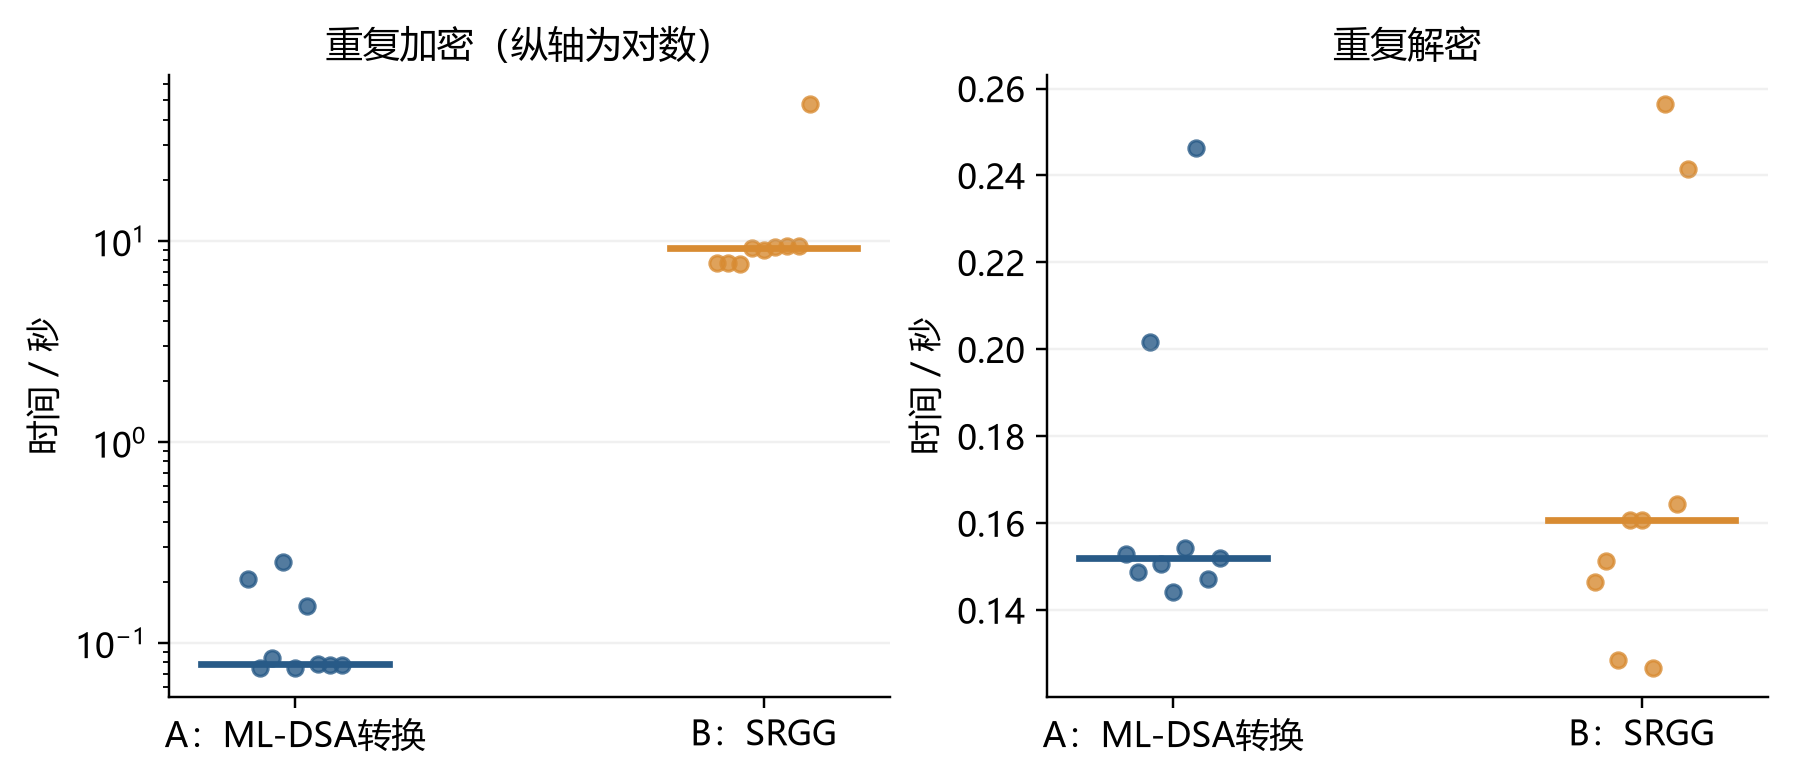
\includegraphics[width=.98\textwidth]{figures/ab-times.png}
\caption{A/B重复操作的时间分布。每组3套系统、每套3次，横线为中位数；加密面板使用对数纵轴}
\label{fig:ab-times}
\end{figure}

各次测量还说明只看中位数会遗漏波动。B有一次重复加密耗时约48.2秒，明显高于其中位数；A也存在较慢观测。首次解密高于重复解密，与叶钥生成有关。恢复对象后，解密回到重复操作相近的量级。

\subsection{对象尺寸与运行内存}
表~\ref{tab:ab-sizes}汇总公共对象、主状态和双方密钥的编码长度。A、B完整密文约139 KiB和146 KiB；本章后面的密文组成分析进一步解释这些字节来自哪里。

\begin{table}[H]
\centering\small
\caption{A/B对象编码长度约值与运行内存}
\label{tab:ab-sizes}
\begin{tabular}{@{}crrrrrr@{}}
\toprule
\rowcolor{black!8} 组 & 公钥 & 主状态 & 发送钥 & 接收状态 & 完整密文 & 内存/MiB \\
\midrule
% BEGIN DATA ab-sizes.tex
A & 14 & 173 & 7.86 & 125 & 139 & 460 \\
B & 46.2 & 262 & 82.4 & 125 & 146 & 485 \\
% END DATA ab-sizes.tex
\bottomrule
\end{tabular}
\begin{minipage}{.96\textwidth}\footnotesize
前五项单位为KiB。对象长度按记录范围取近似值；内存为每10毫秒采样的进程树RSS最高值，包含运行库和子进程，短时峰值可能未被采样捕获。
\end{minipage}
\end{table}

B的公钥、主状态与发送钥大于A，接收状态接近，符合两组共用HIBE而采用不同IBS的结构。编码文件大小和运行内存分别统计：紧凑密钥文件加载后仍会恢复为数学对象，运行时还需要数值库、采样工作区和子进程。

\subsection{C的主要耗时来自委派}
在C的一次32字节消息组合测试中，加密耗时99.0秒，匹配解密425秒，其中Lai委派为393秒，占约92.5\%。这说明对固定通信双方，重复生成同一身份路径的叶钥是优先优化的位置。该次数据来自Ultra 9机器，解密进程存在并发，用于分析其阶段组成。

C的传输密文约4.34 MiB，大部分来自Sageloli签名和Lai胶囊。它展示了另一类HIBE与环IBS在论文配置下的完整组合，以及会话摊销的使用方式。下面分别分析通信量与准备成本。

\subsection{Wang--PW目标档的分阶段运行}

Wang--PW目标档使用$n=512$、$q=4294967291$和$s_0=4$。其密钥和采样工作区远大于常规组合，
因此在128~GiB级服务器上完成目标规模运行。表~\ref{tab:wang-results}汇总已经保存的建立、发钥、
独立签名和LATTE组合结果。

\begin{table}[H]
\centering\small
\caption{Wang--PW目标档与LATTE组合的实测结果}
\label{tab:wang-results}
\begin{tabularx}{\textwidth}{@{}p{.28\textwidth}rX@{}}
\toprule
\rowcolor{black!8} 项目 & 结果 & 说明 \\
\midrule
Setup & 536.63 s & 生成目标档公开矩阵和根陷门 \\
公开参数 & 67,109,371 B & 规范二进制对象 \\
主状态 & 603,980,295 B & 保存紧凑根陷门与参数 \\
KeyExtract & 5,431.95 s & 为一个64字节身份生成用户陷门 \\
用户签名密钥 & 2,214,593,131 B & 规范二进制对象 \\
独立Sign & 175.79 s、175.15 s & 两次恢复后的新消息签名均通过公开验签 \\
签名 & 393,320 B & 包含身份盐、消息盐和短原像 \\
签名峰值RSS & 约41.3 GiB & 进程树采样峰值 \\
LATTE＋Wang加密 & 192.54 s & 78字节应用消息，包含一次新Wang签名 \\
匹配解密 & 2.85 s & 从恢复的接收状态完成诚实解密 \\
完整密文 & 529,207 B & Hybrid与完整字节认证后的wire长度 \\
组合驱动总时长 & 254.86 s & 含准备、一次加密、诚实解密和错误输入检查 \\
\bottomrule
\end{tabularx}
\end{table}

目标档实验分阶段保存并复用已经生成的根和用户密钥。Setup、KeyExtract来自较早的目标生命周期，
最终两次签名与LATTE组合使用修订后的签名实现；表中按阶段呈现这些结果，不把它们相加成一次
连续生命周期。

从使用过程看，Setup和KeyExtract适合放在发钥机构的离线阶段。发送端一次签名约176秒，并需要
约41.3~GiB峰值内存，是组合加密的主要成本。接收端只进行公开验签与LATTE解封装，诚实解密约
2.85秒。393,320字节IBS签名进入对称载荷后，完整密文约517~KiB，明显小于用户签名密钥，
但仍高于A、B。

这一结果表明通用框架能够容纳大对象矩阵SIS后端，同时也说明它更适合低频签名、离线发钥和
资源充足的发送端。三组代表保持A、B、C不变，Wang--PW作为目标规模补充方案单独展示。

\section{小消息为什么仍产生较大的密文}
\subsection{完整密文的组成}
混合加密使应用消息不再受HIBE短明文容量直接限制，但种子胶囊、IBS签名和一次性认证仍需要传输。依据现有安装运行记录与实际编码格式，可将A的一条32字节消息和C的一条空消息分解为表~\ref{tab:ciphertext-parts}。

\begin{table}[H]
\centering\small
\caption{两条已有密文的字节组成核算}
\label{tab:ciphertext-parts}
\begin{tabular}{@{}lrr@{}}
\toprule
\rowcolor{black!8} 组成部分 & A：消息32 B & C：空消息 \\
\midrule
一次性公钥 & 65,536 & 65,536 \\
一次性签名 & 32,768 & 32,768 \\
IBS签名 & 6,237 & 3,227,824 \\
HIBE胶囊 & 37,088 & 1,228,844 \\
应用消息 & 32 & 0 \\
上下文、格式、nonce与标签 & 432 & 432 \\
\midrule
合计 & 142,093 & 4,555,404 \\
\bottomrule
\end{tabular}
\begin{minipage}{.96\textwidth}\footnotesize
整包长度来自已有运行；固定字段按序列化模块核算，HIBE胶囊长度由整包扣除其他组成得到。该核算没有新增加密实验。
\end{minipage}
\end{table}

\begin{figure}[H]
\centering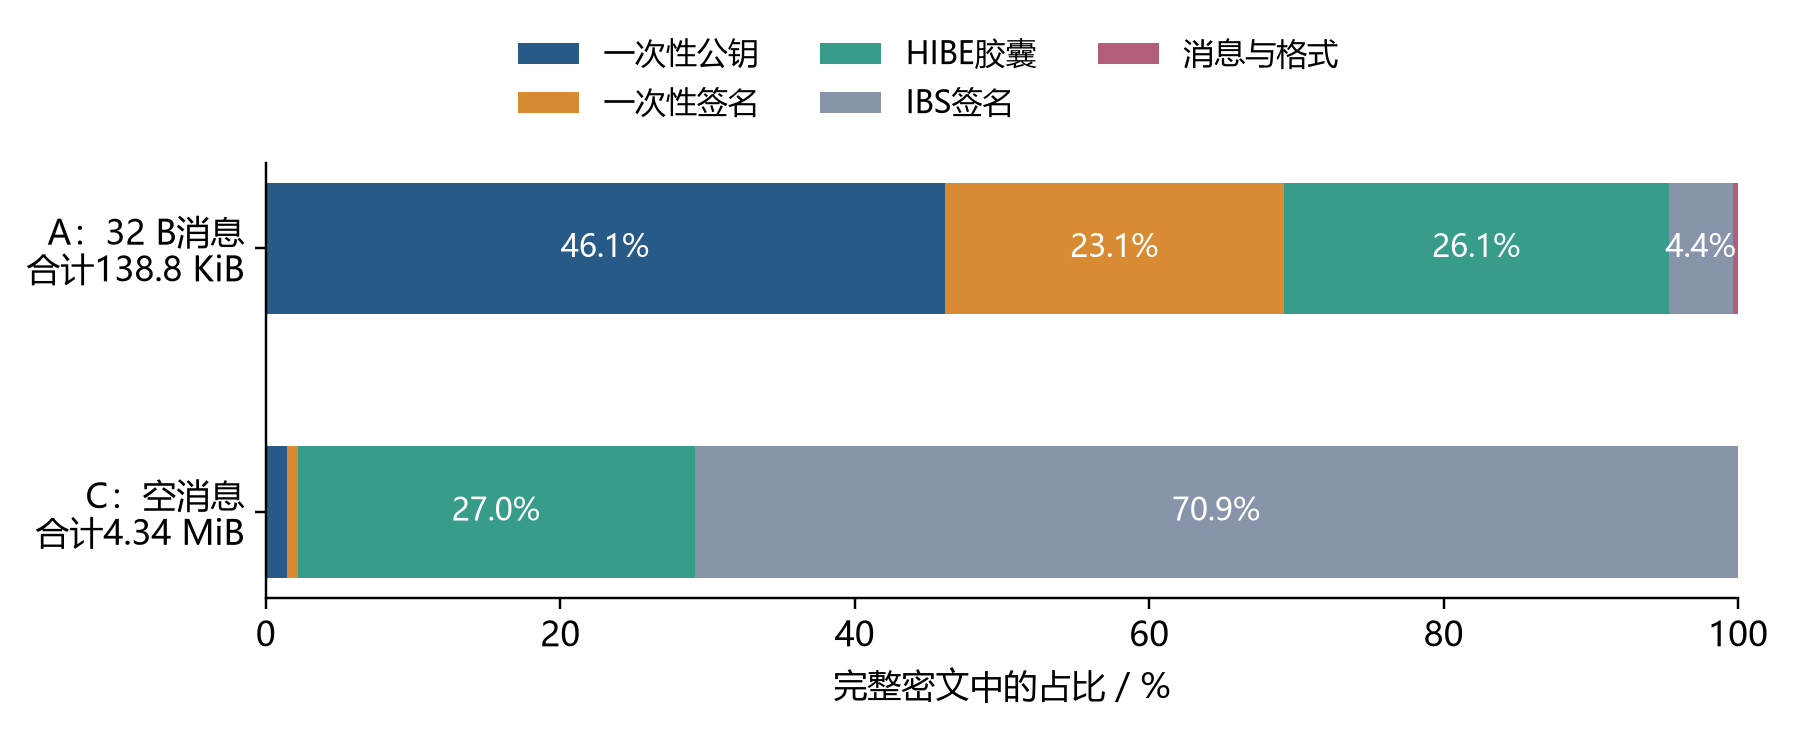
\includegraphics[width=.98\textwidth]{figures/ciphertext-parts.png}
\caption{完整密文的主要成本来源：A以一次性认证为主，C以IBS签名和HIBE胶囊为主}
\label{fig:ciphertext-parts}
\end{figure}

Lamport一次性公钥含1,024个64字节哈希像，签名含512个64字节原像，两项合计固定96 KiB，约占这条A密文的69.2\%。因此，缩短几字节应用消息几乎不会改变A的整包长度。C的IBS签名约占70.9\%，HIBE胶囊约占27.0\%；其后续通信优化应优先考察这两部分。

这也解释了SRGG签名紧凑编码与完整B密文的关系：签名字段变短会减少对称载荷，但整包还包含与A相同的一次性认证结构和LATTE胶囊。评价编码时应同时看单体对象与完整协议中的占比。

\subsection{消息长度与可用容量}
安装运行测试已完成A的0、32、1,024和59,191字节消息，B的0、32、1,024和65,364字节消息；超过应用上限1字节时，系统在生成新密文前拒绝。该批最大长度密文约为197 KiB和210 KiB。

C已完成空消息和1,024字节消息，两条密文相差1,024字节，符合固定胶囊与签名加上可变应用载荷的组成。C的3,924字节上限来自容量计算，尚缺该最大长度的加密解密记录。上述容量检查使用签名保守上界，具体签名和胶囊的编码长度仍可能随随机输出变化。

\section{三项主要优化的效果}
\subsection{结构化采样使论文规模进入实际运行}
Sageloli两个参数档均完成建立、身份发钥、两次签名和验证。表~\ref{tab:sageloli-times}给出各档一套系统的运行记录。

\begin{table}[H]
\centering\small
\caption{Sageloli结构化实现的实际运行，时间单位为秒}
\label{tab:sageloli-times}
\begin{tabular}{@{}lrrrrrr@{}}
\toprule
\rowcolor{black!8} 参数档 & 建立 & 发钥 & 首次签名 & 后续签名 & 验证 & RSS/GiB \\
\midrule
% BEGIN DATA sageloli-times.tex
PARAM-I & 4.99 & 85.1 & 9.28 & 2.02 & 0.517 & 1.36 \\
PARAM-II & 43.6 & 520 & 38.6 & 5.02 & 1.36 & 6.19 \\
% END DATA sageloli-times.tex
\bottomrule
\end{tabular}
\end{table}

PARAM-I发钥约85.1秒，记录峰值RSS约1.36 GiB；PARAM-II发钥约520秒，约6.19 GiB。首次签名明显高于第二次，与同一身份陷门下数值准备的复用相符。结构化实现的主要成果是让这些参数下的采样与验证能够实际完成。稠密矩阵的1.18 TiB是第4章按表示方式计算的存储估算，实验记录对应结构化实现。

\subsection{紧凑编码的收益集中在大整数对象}
图~\ref{fig:codec}和表~\ref{tab:codec-sizes}展示三档SRGG相同数学对象的两种编码。每档独立建立3套系统，在同一对象上交替执行两种格式的编解码。

\begin{figure}[H]
\centering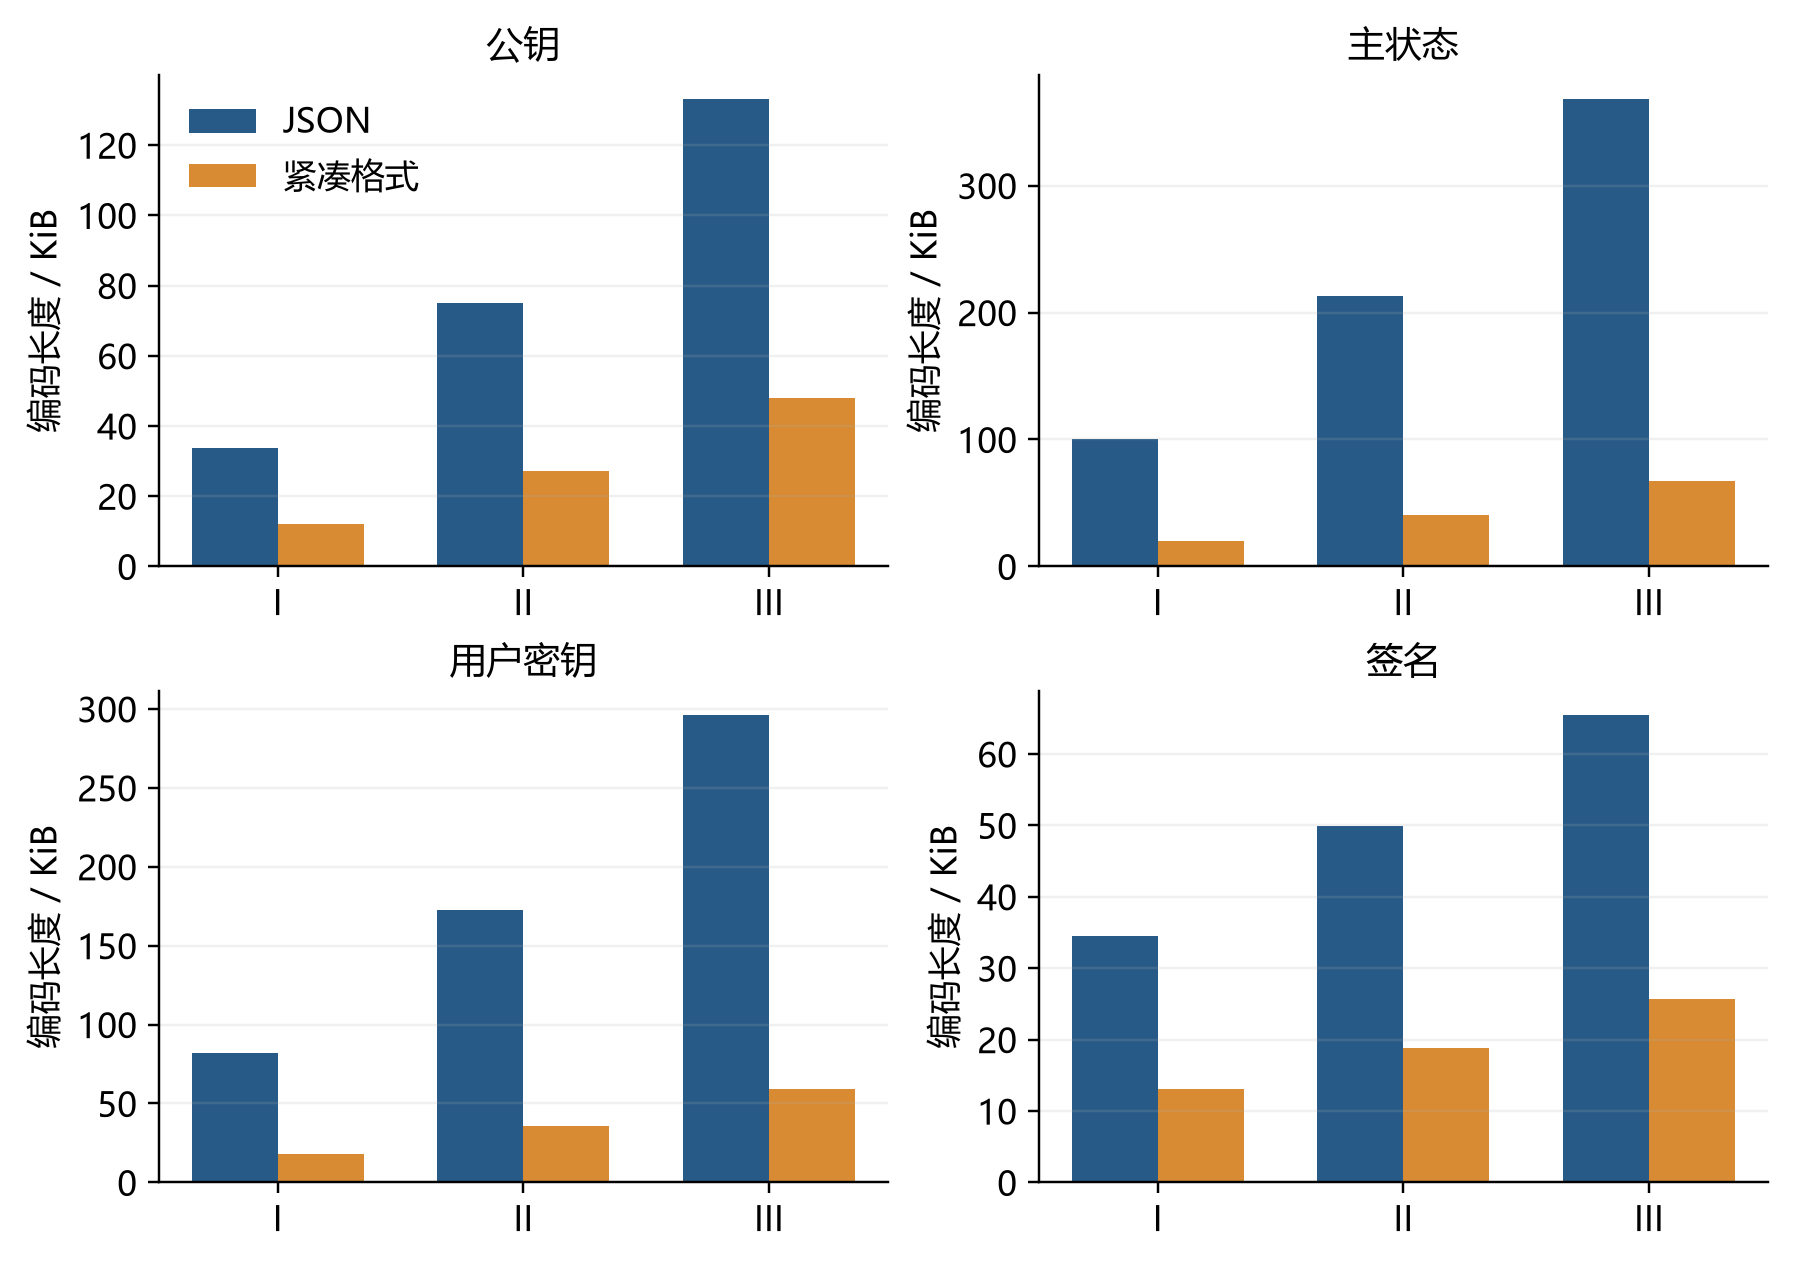
\includegraphics[width=.96\textwidth]{figures/codec.png}
\caption{SRGG三档参数的四类对象尺寸；I、II、III表示参数档}
\label{fig:codec}
\end{figure}

\begin{table}[H]
\centering\small
\caption{SRGG对象编码长度，单位为KiB}
\label{tab:codec-sizes}
\begin{tabular}{@{}lrrrr@{}}
\toprule
\rowcolor{black!8} 参数档／格式 & 公钥 & 主状态 & 用户钥 & 签名 \\
\midrule
% BEGIN DATA codec-sizes.tex
I／JSON & 33.7 & 100 & 82.2 & 34.5 \\
I／紧凑 & 12.1 & 19.8 & 17.8 & 13.1 \\
II／JSON & 75.2 & 213 & 173 & 49.9 \\
II／紧凑 & 27.1 & 40.1 & 35.6 & 18.8 \\
III／JSON & 133 & 368 & 296 & 65.5 \\
III／紧凑 & 48.1 & 67.5 & 59.5 & 25.6 \\
% END DATA codec-sizes.tex
\bottomrule
\end{tabular}
\end{table}

公钥长度缩小约2.77至2.79倍，主状态5.05至5.46倍，用户钥4.61至4.98倍，签名2.55至2.65倍。主状态包含较多小范围陷门系数，去除十进制和结构符号开销后，缩减最明显。

紧凑格式需要位打包、取值检查和规范解码。例如PARAM-I主状态的紧凑编码与解码阶段中位时间约23.1和61.3毫秒，JSON约0.974和37.3毫秒。该项优化的主要收益是对象存储与传输长度，适用于重视密钥保存和通信量的使用方式。

\subsection{接收会话把准备成本分摊到连续消息}
Lai会话实验使用一套主密钥，原路径解密2次，建立会话1次，会话内解密3次。原解密中位数为526秒，会话准备约510秒，后续解密中位数为28.6秒，额外保留叶钥编码34.7 MiB。

\begin{figure}[H]
\centering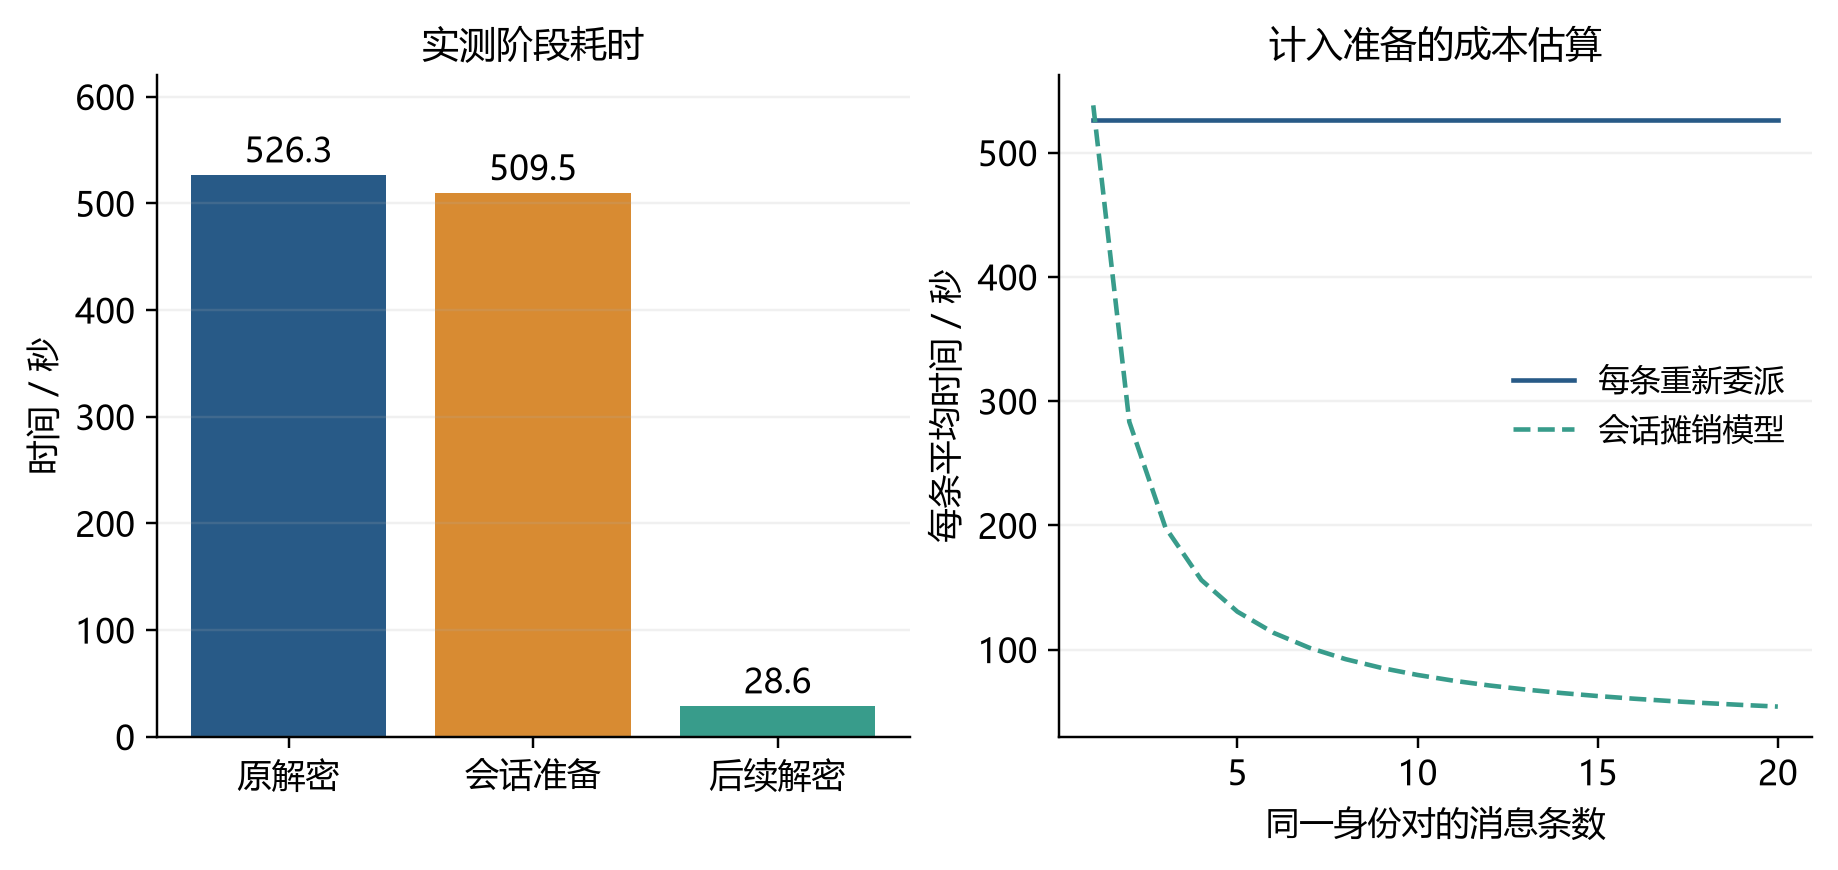
\includegraphics[width=.98\textwidth]{figures/session.png}
\caption{Lai接收会话：左图为测得阶段耗时，右图由阶段中位数代入成本公式估算}
\label{fig:session}
\end{figure}

准备完成后的单条时间约为原路径的$1/18.4$。把准备计入后，首条平均成本约538秒；按$\bar T(N)$模型，处理10条和100条消息时约为79.5秒和33.7秒。右图使用已有阶段耗时外推消息数量，未逐条执行整条曲线。

会话方法把主要委派开销移到首次使用，适合固定身份对的连续消息。短暂的一次通信仍要承担完整准备；长期会话则以额外秘密状态换取较低的后续延迟。该组样本来自一套系统，后续扩大测量可进一步观察不同主密钥下的波动。

\section{缓存与部署位置的完整流程对照}
\subsection{局部缓存对总耗时的影响}
在A、B各3套系统中，分别开启和关闭优化，以相同输入执行完整流程。A缓存机构证书的成功验证结果，原生验签调用由每条2次减少为1次，解密时间比中位数为1.086，逐套范围0.992至1.339。B复用签名数值准备，加密时间比中位数1.030，范围1.009至1.921。

这些结果说明，减少一次局部调用后，总时间仍受其余密码运算与运行波动影响。A有一套测量略微回退，B的中位收益较小。因此，系统保留缓存容量与关闭选项，主要优化结论仍以结构表示、编码和Lai会话为重点。

\subsection{同一运行时下比较文件位置}
三路部署对照固定参数、状态和原生引擎，均由同一WSL Python运行，分别使用Windows盘源码、Windows盘安装包及Linux盘同一安装包。每路完成30次完整加密和30次解密，图~\ref{fig:placement}给出中位数。

\begin{figure}[H]
\centering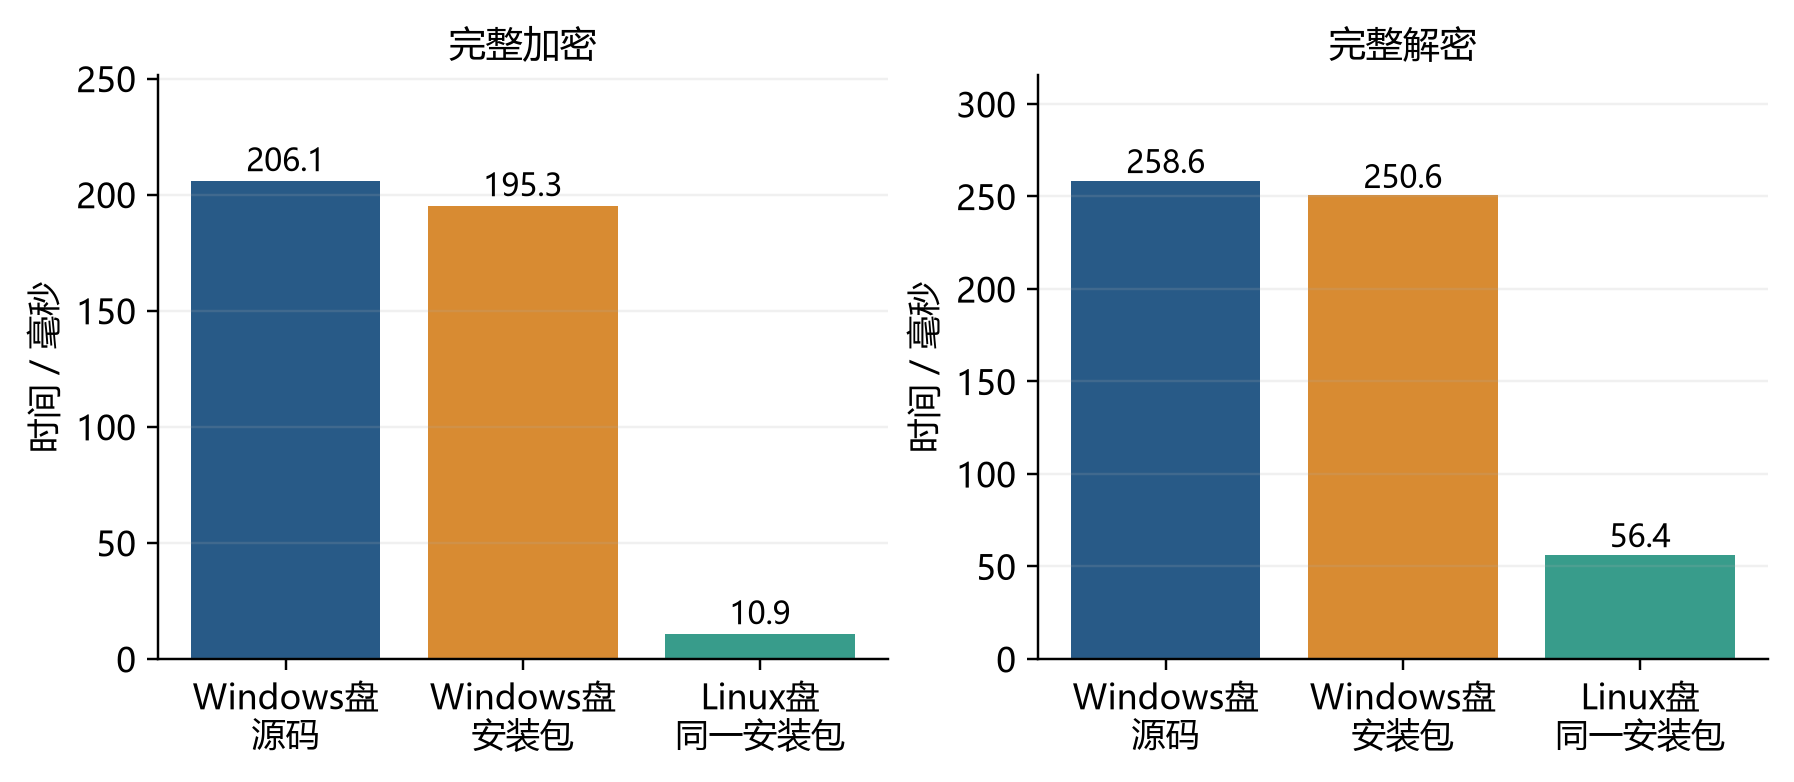
\includegraphics[width=.98\textwidth]{figures/placement.png}
\caption{文件放置位置对完整A流程的影响；三路均使用同一WSL运行时}
\label{fig:placement}
\end{figure}

Linux盘安装包相比Windows盘源码，加密与解密时间比分别约18.87和4.59；只比较同一安装包的两种位置，时间比约17.88和4.45。剖析显示，5次加密的515次文件读取在挂载目录累计约1.073秒，在Linux本地约0.011秒。文件访问是该批运行的重要成本，本机部署优先采用Linux本地目录。

\section{功能测试结果}
三组均完成双方匹配恢复和三类身份错配拒绝。表~\ref{tab:functional}汇总主要检查；另有A的随机身份与消息批次，独立建立3套系统、测试12组输入，60/60项判断符合预期。

\begin{table}[H]
\centering\small
\caption{三组完整协议的主要功能结果}
\label{tab:functional}
\begin{tabularx}{\textwidth}{@{}Xccc@{}}
\toprule
\rowcolor{black!8} 检查情况 & A & B & C \\
\midrule
双方身份匹配 & 恢复原文 & 恢复原文 & 恢复原文 \\
仅接收身份不匹配 & 拒绝 & 拒绝 & 拒绝 \\
仅期望发送身份不匹配 & 拒绝 & 拒绝 & 拒绝 \\
双方身份都不匹配 & 拒绝 & 拒绝 & 拒绝 \\
密文字节修改、截断、追加或重复字段 & 拒绝 & 拒绝 & 拒绝 \\
外层认证有效、内部签名无效 & 拒绝 & 拒绝 & 拒绝 \\
新进程加载对象后解密 & 成功 & 成功 & 成功 \\
\bottomrule
\end{tabularx}
\end{table}

身份错配测试覆盖接收者、发送者和双方同时错误，分别触发不同层次的拒绝。密文字节修改、截断、
追加和重复字段覆盖外层认证与规范解析；“外层认证有效、内部签名无效”则单独检查IBS身份认证。
新进程恢复测试重新加载公开对象和角色密钥，再对已有密文解密，覆盖持久对象的完整使用路径。

\section{本章小结}

实验展示了不同组合的成本分布。A的在线收发最快，B的主要时间集中在发送端SRGG签名，C的主要
时间集中在Lai叶钥委派；Wang--PW的Setup、发钥和签名需要服务器级资源，但接收端解密保持在
数秒量级。三项主要优化分别降低了Sageloli采样内存、SRGG对象尺寸和Lai连续解密延迟。

通信量分析表明，A的密文主要由一次性认证构成，C主要由IBS签名和HIBE胶囊构成。对象级优化
能否明显缩短完整密文，取决于目标字段在整包中的占比。功能测试与恢复测试进一步确认，同一套
协议在A、B、C以及十种常规组合中保持一致的身份匹配和字节处理流程。

\chapter{总结与展望}

\section{工作总结}

本作品围绕“接收者正确、发送者也正确”这一通信需求，完成了抗量子身份基匹配加密的通用设计、
多算法实现和系统优化。发送者用身份指定接收对象，接收者在解密时指定认可的发送来源；两项
身份同时匹配，系统才恢复消息。

协议以两层匿名HIBE控制身份路径，以IBS认证发送者。32字节随机种子解决HIBE短明文与大签名、
长消息之间的容量矛盾；HKDF和AES-256-GCM承担应用载荷；一次性公钥承诺与外层签名把内部身份
认证连接到完整密文字节。建立、双方发钥、加密和匹配解密五个算法在所有组合中保持一致。

软件层将HIBE、IBS、组合配置、公共协议、状态管理和应用入口分开。两种HIBE与五种常规IBS
形成十种端到端配对，覆盖NTRU结构、普通矩阵格、环格和模格路线。目标规模Wang--PW进一步
与LATTE完成端到端组合。新增算法通过接口、规范对象和能力声明接入，不需要复制公共协议。

系统已经提供命令行、浏览器演示、固定发钥和跨进程恢复。使用者可以从算法选择开始，完成系统
建立、角色密钥生成、消息发送、身份匹配解密和错误输入测试。公开对象、角色密钥和密文均采用
带版本的规范编码，可以在不同进程间传递。

\section{创新点及实际效果}

作品的创新不只体现在接入算法数量，更体现在如何把数学方案变成可运行、可扩展的完整系统。
表~\ref{tab:innovation-summary}按照“问题—方法—结果—代价”归纳主要工作。

\begin{table}[H]
\centering\small
\caption{主要创新点、结果与使用取舍}
\label{tab:innovation-summary}
\begin{tabularx}{\textwidth}{@{}>{\raggedright\arraybackslash}p{.18\textwidth}>{\raggedright\arraybackslash}p{.29\textwidth}>{\raggedright\arraybackslash}p{.28\textwidth}>{\raggedright\arraybackslash}X@{}}
\toprule
\rowcolor{black!8} 问题 & 方法 & 结果 & 代价或适用方式 \\
\midrule
不同HIBE／IBS难以直接组合 & 独立接口、SuiteConfig、能力预检、短种子Hybrid与统一字节认证 & 十种常规配对和LATTE＋Wang--PW复用同一五算法 & 新后端需实现严格对象并声明容量 \\
Sageloli稠密展开不可承受 & 保留环多项式，逐频率执行低秩平方根与采样计划 & PARAM-I、II均完成建立、发钥、签名和验证；RSS约1.36、6.19 GiB & 需要数值变换计划和精确方程复核 \\
SRGG大整数对象存储冗长 & 按字段范围使用定长、Zigzag、二元位打包 & 主状态缩小5.05--5.46倍，签名缩小2.55--2.65倍 & 编解码增加少量处理时间 \\
Lai固定身份对反复委派 & 接收会话预先生成并验证叶密钥 & 准备约510秒后，后续解密中位数28.6秒 & 额外保存约34.7 MiB会话叶钥 \\
目标规模矩阵SIS对象巨大 & 流式对象、独立有限Gaussian、固定发行与角色导入 & Wang--PW n512完成签验、恢复和LATTE组合 & 用户钥约2.06 GiB，签名约176秒、峰值约41.3 GiB \\
\bottomrule
\end{tabularx}
\end{table}

\textbf{通用设计。} 通用性首先来自密码边界清晰。HIBE只负责两层身份路径和种子封装，IBS只
负责发送身份认证，组合层只使用公开方法和对象字节。LATTE、Lai以及六种IBS可以保留各自的
模数、维度、环和采样方式。容量预检把原语差异提前转化为可计算的应用消息上限。

\textbf{结构化计算。} Sageloli优化从环方程本身出发，不把多项式机械展开为巨型矩阵。PARAM-I
的相关扰动维数达到403,456，完整实矩阵估算约1.18~TiB；逐频率计算把核心分解降为
$65\times65$小矩阵，并在系数域继续执行精确验签关系。

\textbf{对象级优化。} SRGG编码针对四类对象逐字段确定范围。同一数学对象可以在参考JSON与紧凑
二进制之间无损往返。主状态中大量三值陷门系数只占2 bit，签名中的挑战只占1 bit，从而把存储
收益落到实际密钥文件和密文载荷。

\textbf{使用模式优化。} Lai会话区分了“固定身份对的准备”和“每条消息必须执行的认证解密”。
它没有减少每条消息的验签、GCM和字节认证，而是消除同一路径的重复委派。这一方法特别适合
机构内长期连接和固定设备对。

\section{实验结论}

A、B固定同一LATTE HIBE，因此能够直接观察IBS差异。A的重复加密与解密中位数分别为
78.5毫秒和152毫秒，适合交互演示与高频收发。B的重复加密约9.17秒，时间主要花在SRGG签名；
重复解密约161毫秒，与A接近。该结果说明，B的主要成本在发送端而不是接收端。

C更换为Lai C2与Sageloli PARAM-I。一次完整解密约425秒，其中Lai委派约393秒。接收会话把
固定路径的委派移到准备阶段后，后续解密中位数降至28.6秒。C的完整密文约4.34~MiB，主要由
Sageloli签名和Lai胶囊组成。

Wang--PW目标档展示了另一种资源分布。Setup约536.63秒，单用户发钥约5,431.95秒；复用已发
用户密钥后，一次签名约176秒，LATTE组合加密约192.54秒，匹配解密约2.85秒。发送端的签名
和用户密钥是主要开销，接收端仍能在数秒内完成公开验签与解封装。

密文组成分析还指出一个与算法选择同样重要的问题：A组96~KiB固定空间来自Lamport一次性公钥
和签名，占32字节消息密文的约69.2\%。C组则由大尺寸IBS签名和HIBE胶囊主导。后续缩短通信量
时，应根据组合选择不同目标，而不是只压缩应用消息。

\section{后续工作}

下一批实验将在Intel Core Ultra~9 275HX同一台机器、同一运行时和统一输入下，对十种常规组合
各补测10组独立状态。测量将覆盖Setup、双方发钥、首次与重复收发、恢复、对象尺寸和RSS，并把
首轮、热态和恢复后操作分开统计。完成后，实验章将用这组矩阵作为十种组合的统一横向结果，
A、B、C专项实验继续用于解释优化过程。

通信方面，A组最值得继续研究的是替换或压缩当前96~KiB的一次性认证结构，同时保持内部身份
签名与完整密文字节之间的绑定。C组可以进一步压缩Sageloli签名和Lai胶囊，并增加多套独立主
密钥下的会话测量。Wang--PW则适合继续优化用户陷门表示、流式签名准备和发钥资源调度。

应用方面，可以把当前本地发钥机构扩展为独立服务，由业务系统完成账户审核和身份字符串映射，
发送端与接收端只持有各自角色对象。现有规范编码、SuiteConfig和角色导入已经提供了这一部署
方式所需的基础。

总体而言，本作品已经从通用密码构造走到多原语、完整协议和可操作软件。不同格结构的方案能够
在同一系统中选择和比较，主要计算与存储瓶颈也有对应的实现方法和实验结果。这些工作为后续
参数完善、统一补测和面向具体场景的部署提供了稳定基础。


\clearpage
\addcontentsline{toc}{chapter}{参考文献}
\begin{thebibliography}{99}
\small

\bibitem{wang2024ibme}
Yuejun Wang, Baocang Wang, Qiqi Lai, and Yu Zhan.
Identity-based Matchmaking Encryption with Stronger Security and Instantiation on Lattices.
\emph{Theoretical Computer Science}, 2024.
doi: 10.1016/j.tcs.2024.115048.

\bibitem{zhao2024latte}
Raymond K. Zhao, Sarah McCarthy, Ron Steinfeld, Amin Sakzad, and Máire O'Neill.
Quantum-safe HIBE: Does It Cost a LATTE?
\emph{IEEE Transactions on Information Forensics and Security}, 2023.

\bibitem{lai2015trapdoors}
Russell W. F. Lai, Henry K. F. Cheung, and Sherman S. M. Chow.
Trapdoors for Ideal Lattices with Applications.
In \emph{Inscrypt 2014}, LNCS 8957, pp. 239--256, 2015.
doi: 10.1007/978-3-319-16745-9\_14.

\bibitem{jia2025ibs}
Huiwen Jia, Ying Liu, Chunming Tang, and Lin Wang.
Constructing Efficient Identity-Based Signatures on Lattices.
\emph{IET Information Security}, 2025.
doi: 10.1049/ise2/6684889.

\bibitem{sageloli2023ibs}
Éric Sageloli, Pierre Pébereau, Pierrick Méaux, and Céline Chevalier.
Shorter and Faster Identity-Based Signatures with Tight Security in the (Q)ROM from Lattices.
In \emph{ACNS 2023}, 2023.
doi: 10.1007/978-3-031-33488-7\_24.

\bibitem{pan2021ibs}
Jiaxin Pan and Benedikt Wagner.
Short Identity-Based Signatures with Tight Security from Lattices.
In \emph{PQCrypto 2021}, 2021.
ePrint 2021/970.

\bibitem{galindo2006ibs}
David Galindo, Javier Herranz, and Eike Kiltz.
On the Generic Construction of Identity-Based Signatures with Additional Properties.
In \emph{ASIACRYPT 2006}, 2006.

\bibitem{nist2024fips204}
National Institute of Standards and Technology.
\emph{Module-Lattice-Based Digital Signature Standard}.
FIPS 204, 2024.

\bibitem{micciancio2012trapdoors}
Daniele Micciancio and Chris Peikert.
Trapdoors for Lattices: Simpler, Tighter, Faster, Smaller.
In \emph{EUROCRYPT 2012}, 2012.

\bibitem{lpr2013ring}
Vadim Lyubashevsky, Chris Peikert, and Oded Regev.
On Ideal Lattices and Learning with Errors over Rings.
\emph{Journal of the ACM}, 60(6), 2013.

\bibitem{langlois2015module}
Adeline Langlois and Damien Stehl\'e.
Worst-Case to Average-Case Reductions for Module Lattices.
\emph{Designs, Codes and Cryptography}, 75, pp. 565--599, 2015.

\bibitem{rfc5869}
Hugo Krawczyk and Pasi Eronen.
HMAC-based Extract-and-Expand Key Derivation Function (HKDF).
RFC 5869, 2010.

\bibitem{nist2007gcm}
National Institute of Standards and Technology.
\emph{Recommendation for Block Cipher Modes of Operation: Galois/Counter Mode (GCM) and GMAC}.
Special Publication 800-38D, 2007.

\bibitem{lamport1979ots}
Leslie Lamport.
Constructing Digital Signatures from a One Way Function.
SRI International, CSL-98, 1979.

\bibitem{luo2024ibs}
Pingbin Luo, Xinjian Chen, Willy Susilo, and Qiong Huang.
Identity-Based Signature from Lattices without Trapdoors.
In \emph{ICICS 2024}, 2024.

\bibitem{falcon2020}
Pierre-Alain Fouque et al.
\emph{Falcon: Fast-Fourier Lattice-based Compact Signatures over NTRU}.
Specification v1.2, 2020.

\end{thebibliography}

\end{document}
